\documentclass[11pt,a4paper]{article}

\usepackage[T1]{fontenc}
\usepackage[utf8]{inputenc}
\usepackage[spanish,es-noquoting,es-tabla]{babel}
\usepackage{amsmath,amssymb,amsthm}
\usepackage{mathtools}
\usepackage{csquotes}
\usepackage{array}
\usepackage{booktabs}
\usepackage{graphicx}
\usepackage{longtable}
\usepackage{caption}
\usepackage{subcaption}
\usepackage{enumitem}
\usepackage[margin=2.4cm]{geometry}
\usepackage{microtype}
\usepackage{xcolor}
\setlength{\emergencystretch}{3em}
\usepackage[colorlinks=true,linkcolor=blue!55!black,citecolor=blue!55!black,
            urlcolor=blue!55!black]{hyperref}

\graphicspath{{../plots/}{../gpu_vs_cpu/}{figs_forward/}}

\newcommand{\vect}[1]{\boldsymbol{#1}}
\newcommand{\matr}[1]{\mathbf{#1}}
\newcommand{\code}[1]{\texttt{#1}}
\newcommand{\dd}{\mathrm{d}}
\DeclareMathOperator{\Cov}{Cov}
\DeclareMathOperator*{\E}{\mathbb{E}}

\theoremstyle{definition}
\newtheorem{obs}{Observación}
\newtheorem{salvedad}{Salvedad}

\theoremstyle{plain}
\newtheorem{prop}{Proposición}

\title{\textbf{El \emph{forward} completo del \emph{pipeline} CRB}\\[2mm]
\large De la simulación del transitorio a las elipses de incertidumbre,\\
con la justificación de cada paso}
\author{Repositorio \code{crb} --- rama consolidada}
\date{3 de septiembre de 2026}

\begin{document}
% babel-spanish activa el caracter de comillas dobles como abreviatura; hay que
% desactivarla para poder citar literales de Python.
\shorthandoff{"}
\maketitle

\begin{abstract}
Estas notas explican, de principio a fin y sin saltos, todo el \emph{forward} del
\emph{pipeline} actual del repositorio: el simulador vectorizado en PyTorch
(\code{simulator.py}), el modelo estadístico de Poisson que se le acopla, el
jacobiano por diferencias finitas, la información de Fisher, la cota de
Cramér--Rao y las elipses de incertidumbre que se dibujan al final, con la
grilla de referencia de $32\times32$ píxeles. Cada fórmula va seguida de su
justificación: por qué ese término, por qué esa decisión de implementación y qué
pasaría si no estuviera. Todas las expresiones se han verificado contra el
código, y cada paso cita el archivo y la función donde vive.

Cuatro resultados de la verificación merecen adelantarse, porque corrigen ideas
que circulan sobre este código. Primero, \code{facet.obj} es un cuadrilátero
\emph{plano} de dos triángulos con extensión nula en $z$, de modo que la rama
$1.1/\text{extents}_z$ del factor de escala \textbf{nunca se activa} y la faceta
acaba midiendo $0.5\times1.585\,$m. Segundo, la densificación no deja $10\,000$
triángulos sino $\mathbf{32\,768}$, porque $10\,000$ es un piso y cada
subdivisión cuadruplica. Tercero, el \emph{pitch} de $1.57$ rad no es
exactamente $\pi/2$, así que la normal de la faceta queda inclinada
$0.0456^\circ$ respecto de la horizontal. Y cuarto, el \code{np.roll} final es
una permutación cíclica de los píxeles y por tanto \textbf{deja la información
de Fisher exactamente invariante}: se demuestra en la
proposición~\ref{prop:roll} y se comprueba numéricamente a precisión de máquina.
\end{abstract}

\tableofcontents

%=======================================================================
\section{Planteamiento y notación}
\label{sec:planteamiento}

\subsection{La escena}

La geometría es la de una \emph{cámara de esquina}. Todo vive en un sistema de
coordenadas con el suelo en $z=0$:

\begin{itemize}[leftmargin=*]
  \item Un \textbf{láser} pulsado está en el origen $\vect p_\ell=(0,0,0)$,
        apuntando hacia arriba con normal $\vect n_\ell=(0,0,1)$
        (\code{laser\_pos}, \code{laser\_normal} en
        \code{simulator.simulation}). El punto del suelo que ilumina se comporta
        como un emisor difuso secundario.
  \item Una \textbf{arista ocluyente} coincide con la recta $y=0$: el
        semiplano $x<0$ está tapado por la pared de la esquina y el semiplano
        $x>0$ es el hueco por el que la luz puede pasar. Esta convención no está
        escrita como una geometría explícita en el código, sino \emph{implícita}
        en el test de oclusión de la sección~\ref{sec:oclusion}.
  \item Un \textbf{sensor SPAD} observa un parche del suelo: un cuadrado de
        \code{camera\_FOV}$=0.25\,$m de lado, centrado en
        \code{camera\_FOV\_center}$=(0,-\text{FOV}/2,0)=(0,-0.125,0)$, dividido
        en $N\times N$ píxeles con $N=$\code{cam\_pixel\_dim}$=32$.
  \item Una \textbf{faceta oculta} (\code{facet.obj}) de anchura
        $w=0.5\,$m está detrás de la arista, en el lado $y>0$.
\end{itemize}

Los centros de píxel se construyen en \code{simulate\_transient\_torch} con dos
\code{linspace} que dejan medio píxel de margen en cada borde:
%
\begin{equation}
\label{eq:grid}
x_j = -\frac{\text{FOV}}{2}+\frac{\text{FOV}}{2N}+j\,\frac{\text{FOV}}{N},
\qquad
y_i = -\text{FOV}+\frac{\text{FOV}}{2N}+i\,\frac{\text{FOV}}{N},
\qquad i,j=0,\dots,N-1 .
\end{equation}
%
El \emph{pitch} de píxel es por tanto
%
\begin{equation}
\label{eq:pitch}
\Delta_{\text{px}} = \frac{\text{FOV}}{N} = \frac{0.25\,\text{m}}{32}
= 7.8125\,\text{mm}.
\end{equation}

\begin{obs}[El \emph{pitch} de la grilla \emph{baseline} es $7.81\,$mm, no
$3.9\,$mm]
\label{obs:pitch}
Es fácil confundirse aquí, porque $3.9$ aparece dos veces en la configuración
por motivos distintos: $3.9\,$mm era el \emph{pitch} de la grilla \emph{antigua}
de $64\times64$ ($0.25/64$), y $\Delta t = 3.9\cdot10^{-10}\,$s es el tamaño de
\emph{bin} temporal. Con la grilla \emph{baseline} de $32\times32$ el
\emph{pitch} es el doble, $7.8125\,$mm. La coincidencia numérica es casualidad.
\end{obs}

El eje temporal se discretiza en \emph{bins} de
$\Delta t=$\code{bin\_size}$=3.9\cdot10^{-10}\,$s. Lo que importa es la longitud
de camino que cabe en un \emph{bin}:
%
\begin{equation}
\label{eq:cdt}
c\,\Delta t = 299\,792\,458\ \tfrac{\text{m}}{\text{s}}
\times 3.9\cdot10^{-10}\,\text{s} = 0.116919\,\text{m}
\approx 11.7\,\text{cm de camino recorrido}.
\end{equation}
%
Esta cifra reaparecerá constantemente: es la resolución bruta del sensor y la
fuente del principal problema numérico del \emph{pipeline}
(sección~\ref{sec:fd}).

\subsection{Los parámetros a estimar}

La pose de la faceta se describe en coordenadas polares sobre el suelo por
%
\begin{equation}
\label{eq:psi}
\vect\psi = (\rho,\varphi),
\qquad
\text{posición} = (\rho\cos\varphi,\ \rho\sin\varphi,\ 0),
\end{equation}
%
y la faceta se coloca de pie, con la normal apuntando hacia el origen dentro del
plano horizontal:
%
\begin{equation}
\label{eq:normal}
\vect n(\varphi) = (-\cos\varphi,\ -\sin\varphi,\ 0).
\end{equation}
%
La sección~\ref{sec:placement} demuestra que la cadena de rotaciones del código
produce exactamente esta normal.

\begin{obs}[Por qué polares y no cartesianas]
La geometría del problema es radial: el láser está en el origen y la arista
ocluyente pasa por él. El tiempo de vuelo depende esencialmente de $\rho$ (la
distancia) y la oclusión depende esencialmente de $\varphi$ (el ángulo respecto
del hueco). Separar el problema en \enquote{cuán lejos} y \enquote{en qué
dirección} desacopla los dos mecanismos físicos de información, y hace que las
elipses de la sección~\ref{sec:elipse} se lean directamente como
\enquote{incertidumbre en rango} frente a \enquote{incertidumbre en azimut}.
\end{obs}

\subsection{Qué queremos calcular}

Con la faceta en $\vect\psi$, el simulador produce un transitorio esperado
$\vect y(\vect\psi)\in\mathbb R^{N\times N\times T}$. Un experimento real
mediría un transitorio \emph{ruidoso}, y de él se querría estimar
$\hat{\vect\psi}$. La pregunta que responden estas notas no es \emph{cómo}
estimar, sino \textbf{cuál es la mejor precisión alcanzable}: la cota de
Cramér--Rao (CRB), que acota por debajo la covarianza de cualquier estimador
insesgado. El recorrido es
%
\[
\underbrace{\vect\psi \longrightarrow \vect y(\vect\psi)}_{\S\ref{sec:sim}}
\longrightarrow
\underbrace{\vect g = \vect y + b}_{\S\ref{sec:estadistico}}
\longrightarrow
\underbrace{\matr J = \partial\vect g/\partial\vect\psi}_{\S\ref{sec:fd}}
\longrightarrow
\underbrace{\matr I = \matr J^\top\!\operatorname{diag}(1/\vect g)\,\matr J}_{\S\ref{sec:fisher}}
\longrightarrow
\underbrace{\matr C=\matr I^{-1}}_{\S\ref{sec:crb}}
\longrightarrow
\underbrace{\text{elipse}}_{\S\ref{sec:elipse}} .
\]

La figura~\ref{fig:esquema} resume la escena y adelanta el test de oclusión.

\begin{figure}[htbp]
\centering
\IfFileExists{figs_forward/esquema_esquina.png}{%
  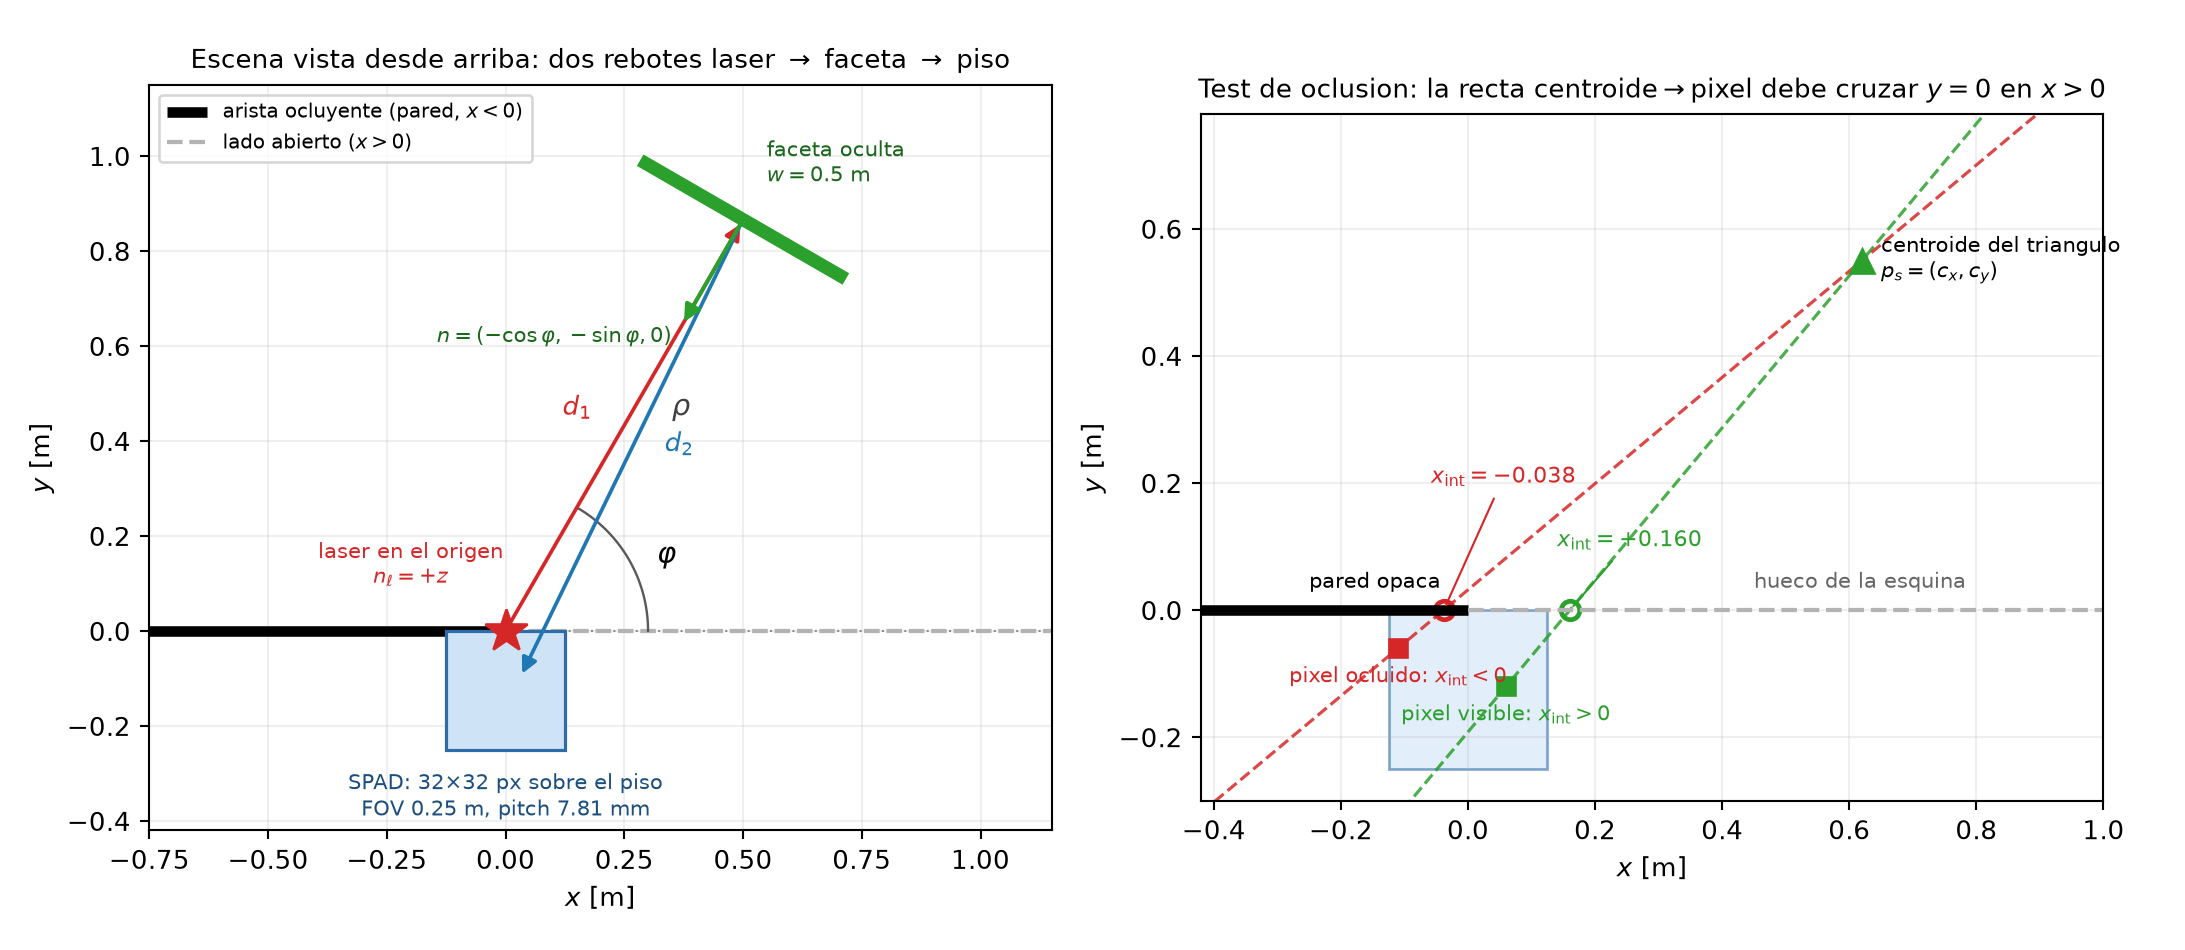
\includegraphics[width=\textwidth]{esquema_esquina.png}}{%
  \fbox{\parbox{0.9\textwidth}{\centering\vspace{2em}
  (figura \code{esquema\_esquina.png} no disponible)\vspace{2em}}}}
\caption{Izquierda: la escena vista desde arriba. El láser en el origen ilumina
el suelo; la luz difundida llega a la faceta oculta (recorrido $d_1$), se
difunde de nuevo y alcanza el parche de suelo que el SPAD observa (recorrido
$d_2$). La arista ocluyente tapa $x<0$. Derecha: el test de oclusión de la
sección~\ref{sec:oclusion}: la recta que une el centroide de un triángulo con un
píxel debe cruzar $y=0$ del lado abierto, $x_{\text{int}}>0$.}
\label{fig:esquema}
\end{figure}

%=======================================================================
\section{La simulación, paso a paso}
\label{sec:sim}

Toda esta sección describe \code{simulator.py}. La malla se coloca en
\code{\_transform\_object\_mesh}, el bucle radiométrico vive en
\code{simulate\_transient\_torch} y \code{simulation} orquesta a los dos.

%-----------------------------------------------------------------------
\subsection{Colocación de la faceta}
\label{sec:placement}

\paragraph{Carga y densificación.}
El archivo \code{objects/facet.obj} es, medido directamente, un
\textbf{cuadrilátero plano de $2$ triángulos y $4$ vértices}, con extensiones
$(0.390656,\ 1.238402,\ 0)\,$m. A continuación
%
\begin{center}
\code{obj = densify\_mesh\_if\_needed(obj, min\_triangles=10000)}
\end{center}
%
subdivide la malla. La subdivisión de \code{trimesh} parte cada triángulo en
cuatro, de modo que el número de triángulos sigue $2\cdot4^k$; el primer $k$ con
$2\cdot4^k\ge10\,000$ es $k=7$, y por tanto
%
\begin{equation}
\label{eq:ntri}
T_{\triangle} = 2\cdot4^7 = 32\,768\ \text{triángulos}.
\end{equation}

\begin{obs}[No son $10\,000$ triángulos, son $32\,768$]
\label{obs:ntri}
\code{min\_triangles} es un \emph{piso}, no un objetivo: la subdivisión no puede
aterrizar en $10\,000$ porque solo sabe cuadruplicar. El documento y cualquier
cálculo de coste deben usar $32\,768$.
\end{obs}

\paragraph{Por qué densificar: la suma es una cuadratura.}
Esta es la justificación central de todo el modelo. La energía que la faceta
reenvía hacia un píxel es una \textbf{integral de superficie} sobre la faceta
$S$,
%
\begin{equation}
\label{eq:integral}
y_{\text{px}} = \int_S f(\vect p_s)\,\dd A(\vect p_s),
\end{equation}
%
con $f$ el integrando radiométrico que se construye en las secciones
siguientes. El simulador la aproxima por una \textbf{regla del punto medio} por
triángulo: evalúa $f$ en el centroide $\vect c_t$ y la pesa por el área
$A_t$,
%
\begin{equation}
\label{eq:cuadratura}
y_{\text{px}} \approx \sum_{t=1}^{T_\triangle} f(\vect c_t)\,A_t .
\end{equation}
%
El error de esta cuadratura decrece al refinar la malla, y hace falta refinar
mucho por dos razones: $f$ contiene $1/d_2^2$ y cosenos, que son no lineales
sobre una faceta de más de un metro y medio de alto; y sobre todo $f$ contiene
un \textbf{indicador de oclusión discontinuo}, de modo que con pocos triángulos
la visibilidad parcial de la faceta se representa muy groseramente. Si no se
densificara ($2$ triángulos), la faceta sería visible o invisible casi en
bloque; con $32\,768$ triángulos la frontera de la sombra queda resuelta
finamente. En la sección~\ref{sec:fd} veremos que esta misma densificación es lo
que hace viable el jacobiano por diferencias finitas.

\paragraph{Escala.}
El código construye una lista de factores candidatos y toma el menor:
%
\begin{equation}
\label{eq:escala}
s = \min\Bigl(\underbrace{\tfrac{w}{\text{extents}_x}}_{\text{si } \text{extents}_x>10^{-12}},\
              \underbrace{\tfrac{1.1}{\text{extents}_z}}_{\text{si } \text{extents}_z>10^{-12}}\Bigr).
\end{equation}
%
Con \code{facet.obj} se tiene $\text{extents}_z=0$ exactamente (es un
cuadrilátero plano en el plano $xy$), así que la guarda
$\text{extents}_z>10^{-12}$ \textbf{descarta el segundo candidato} y sobra
únicamente el primero:
%
\begin{equation}
s = \frac{w}{\text{extents}_x} = \frac{0.5}{0.390656} = 1.279898 .
\end{equation}

\begin{obs}[La cota de $1.1\,$m de alto es inerte para esta faceta]
\label{obs:altura}
Es tentador leer \eqref{eq:escala} como \enquote{la faceta no pasará de
$1.1\,$m}. Con \code{facet.obj} eso es falso: como la malla es plana, la rama de
$z$ no participa, y la faceta escalada acaba midiendo
%
\[
0.5\,\text{m (ancho)} \times 1.585\,\text{m (alto)},
\qquad \text{área}=0.79251\,\text{m}^2,
\]
%
es decir, $1.585 = 1.238402\times1.279898$, bastante por encima de $1.1$. La
cota solo actuaría con un objeto que tuviera espesor en $z$ \emph{antes} de las
rotaciones. Este detalle importa porque el alto de la faceta es lo que dispersa
los tiempos de vuelo (sección~\ref{sec:binning}).
\end{obs}

\paragraph{Rotaciones.}
Se aplican en este orden: \emph{pitch} de $1.57\,$rad alrededor de $x$,
\emph{roll} de $0$ alrededor de $y$, y \emph{yaw} de
$\theta=\varphi+3\pi/2$ alrededor de $z$. El \emph{pitch} pone de pie el
cuadrilátero, que originalmente yace en el plano $xy$ con normal
$\vect n_0=(0,0,1)$:
%
\begin{equation}
\matr R_x(1.57)\,\vect n_0
=\bigl(0,\ -\sin 1.57,\ \cos 1.57\bigr)
=(0,\ -0.99999968,\ 0.00079633).
\end{equation}

\begin{obs}[$1.57 \ne \pi/2$: la faceta queda inclinada $0.0456^\circ$]
\label{obs:pitch157}
Como $\pi/2 = 1.5707963\ldots$, el \emph{pitch} de $1.57$ deja un residuo
$\pi/2-1.57 = 7.96\cdot10^{-4}\,$rad. La normal conserva una componente
$z$ de $\cos(1.57)=7.9633\cdot10^{-4}$, lo que equivale a
$0.0456^\circ$ de desviación respecto de la normal horizontal
ideal~\eqref{eq:normal}. Es un detalle inocuo para el CRB (afecta a los cosenos
en el quinto decimal) pero conviene no presentar $1.57$ como si fuese $\pi/2$
exacto: es un valor \emph{redondeado} heredado de la configuración original.
\end{obs}

\begin{prop}[El \emph{yaw} $\theta=\varphi+3\pi/2$ produce la normal
\eqref{eq:normal}]
\label{prop:yaw}
Sea $\vect n_1=(0,-1,0)$ la normal tras un \emph{pitch} de exactamente
$\pi/2$. Entonces $\matr R_z(\varphi+3\pi/2)\,\vect n_1 = (-\cos\varphi,
-\sin\varphi, 0)$.
\end{prop}

\begin{proof}
Con $\matr R_z(\theta)=\begin{psmallmatrix}\cos\theta&-\sin\theta&0\\
\sin\theta&\cos\theta&0\\0&0&1\end{psmallmatrix}$ se tiene
$\matr R_z(\theta)(0,-1,0)^\top=(\sin\theta,\,-\cos\theta,\,0)^\top$.
Sustituyendo $\theta=\varphi+3\pi/2$ y usando
$\sin(\varphi+3\pi/2)=-\cos\varphi$ y $\cos(\varphi+3\pi/2)=\sin\varphi$,
%
\[
\matr R_z(\varphi+\tfrac{3\pi}{2})(0,-1,0)^\top
=(-\cos\varphi,\ -\sin\varphi,\ 0)^\top . \qedhere
\]
\end{proof}

El desplazamiento de $3\pi/2$ es, entonces, exactamente el necesario para que
\emph{la cara de la faceta mire al origen}, que es lo que interesa: la faceta
debe recibir luz del punto iluminado del suelo y reenviarla, no darle la
espalda. Verificado numéricamente sobre la malla real, la normal media ponderada
por área da $(-0.5,-0.866025,0.000796)$ para $\varphi=60^\circ$, a
$0.0456^\circ$ de la predicción \eqref{eq:normal} --- exactamente el residuo
de la observación~\ref{obs:pitch157}.

\paragraph{Apoyo en el suelo y traslación.}
Finalmente
%
\begin{center}
\code{obj.apply\_translation([0,0,-z\_min])} \quad y luego \quad
\code{obj.apply\_translation(v1)}
\end{center}
%
con \code{v1}$=(\rho\cos\varphi,\rho\sin\varphi,0)$. El primer paso baja la
malla hasta que su vértice más bajo toca $z=0$, y el segundo la lleva a la pose
pedida. El orden importa: primero se apoya en el suelo alrededor del origen y
después se traslada, de forma que la faceta \textbf{siempre queda de pie sobre
el suelo} independientemente de $\rho$ y $\varphi$. Su centroide ponderado por
área queda en $z=0.792514\,$m, la mitad de $1.585$, como corresponde a un
rectángulo uniforme.

%-----------------------------------------------------------------------
\subsection{Las dos distancias y el modelo de dos rebotes}
\label{sec:distancias}

Para cada triángulo con centroide $\vect c_t$ y cada píxel en $\vect q_p$:
%
\begin{align}
\label{eq:d1}
d_1(t) &= \lVert \vect p_\ell - \vect c_t\rVert
        &&\text{\code{lps = laser\_pos - centers}, \code{d1s = sum(lps*lps)}},\\
\label{eq:d2}
d_2(t,p) &= \lVert \vect q_p - \vect c_t\rVert
        &&\text{\code{fovsp = cam\_pos - centers}, \code{d2s = sum(fovsp**2)}} .
\end{align}
%
Nótese que $d_1$ depende solo del triángulo (vector de tamaño $T_\triangle$)
mientras que $d_2$ depende del par (vector $T_\triangle\times P$); el código
explota esa asimetría con \emph{broadcasting}, lo que ahorra memoria.

\paragraph{Por qué dos rebotes y no tres.}
El camino modelado es
%
\[
\text{láser} \xrightarrow{\ d_1\ } \text{faceta oculta}
\xrightarrow{\ d_2\ } \text{parche de suelo} \xrightarrow{\ \text{óptica}\ }
\text{SPAD}.
\]
%
Hay dos \emph{reflexiones difusas} en el trayecto: la del punto iluminado del
suelo (que reemite hacia la faceta) y la de la faceta (que reemite hacia el
suelo observado). El último tramo, del parche de suelo al sensor, \textbf{no es
una reflexión}: el SPAD \emph{mira} directamente ese parche, así que cada píxel
recoge la radiancia del punto del suelo que le corresponde. Por eso no aparece
ni un tercer factor $1/d^2$ ni un quinto coseno. Esta es la diferencia
fundamental con el planteamiento del \emph{writeup} de referencia, que sí
incluye el tramo cámara--suelo y en consecuencia arrastra una constante distinta
(sección~\ref{sec:atenuacion}).

Los rebotes de orden superior (luz que va y vuelve varias veces) se desprecian:
cada reflexión difusa cuesta un factor $\sim1/(\pi d^2)$, y a distancias del
orden del metro eso son dos órdenes de magnitud por rebote. Es la aproximación
estándar en NLOS de tres rebotes, aquí con el tercero absorbido por la óptica
del sensor.

La figura~\ref{fig:geometria} muestra $d_2$, la atenuación y el camino total
sobre la grilla de píxeles.

\begin{figure}[htbp]
\centering
\IfFileExists{../plots/crb_sim_components_gpu_geometry.png}{%
  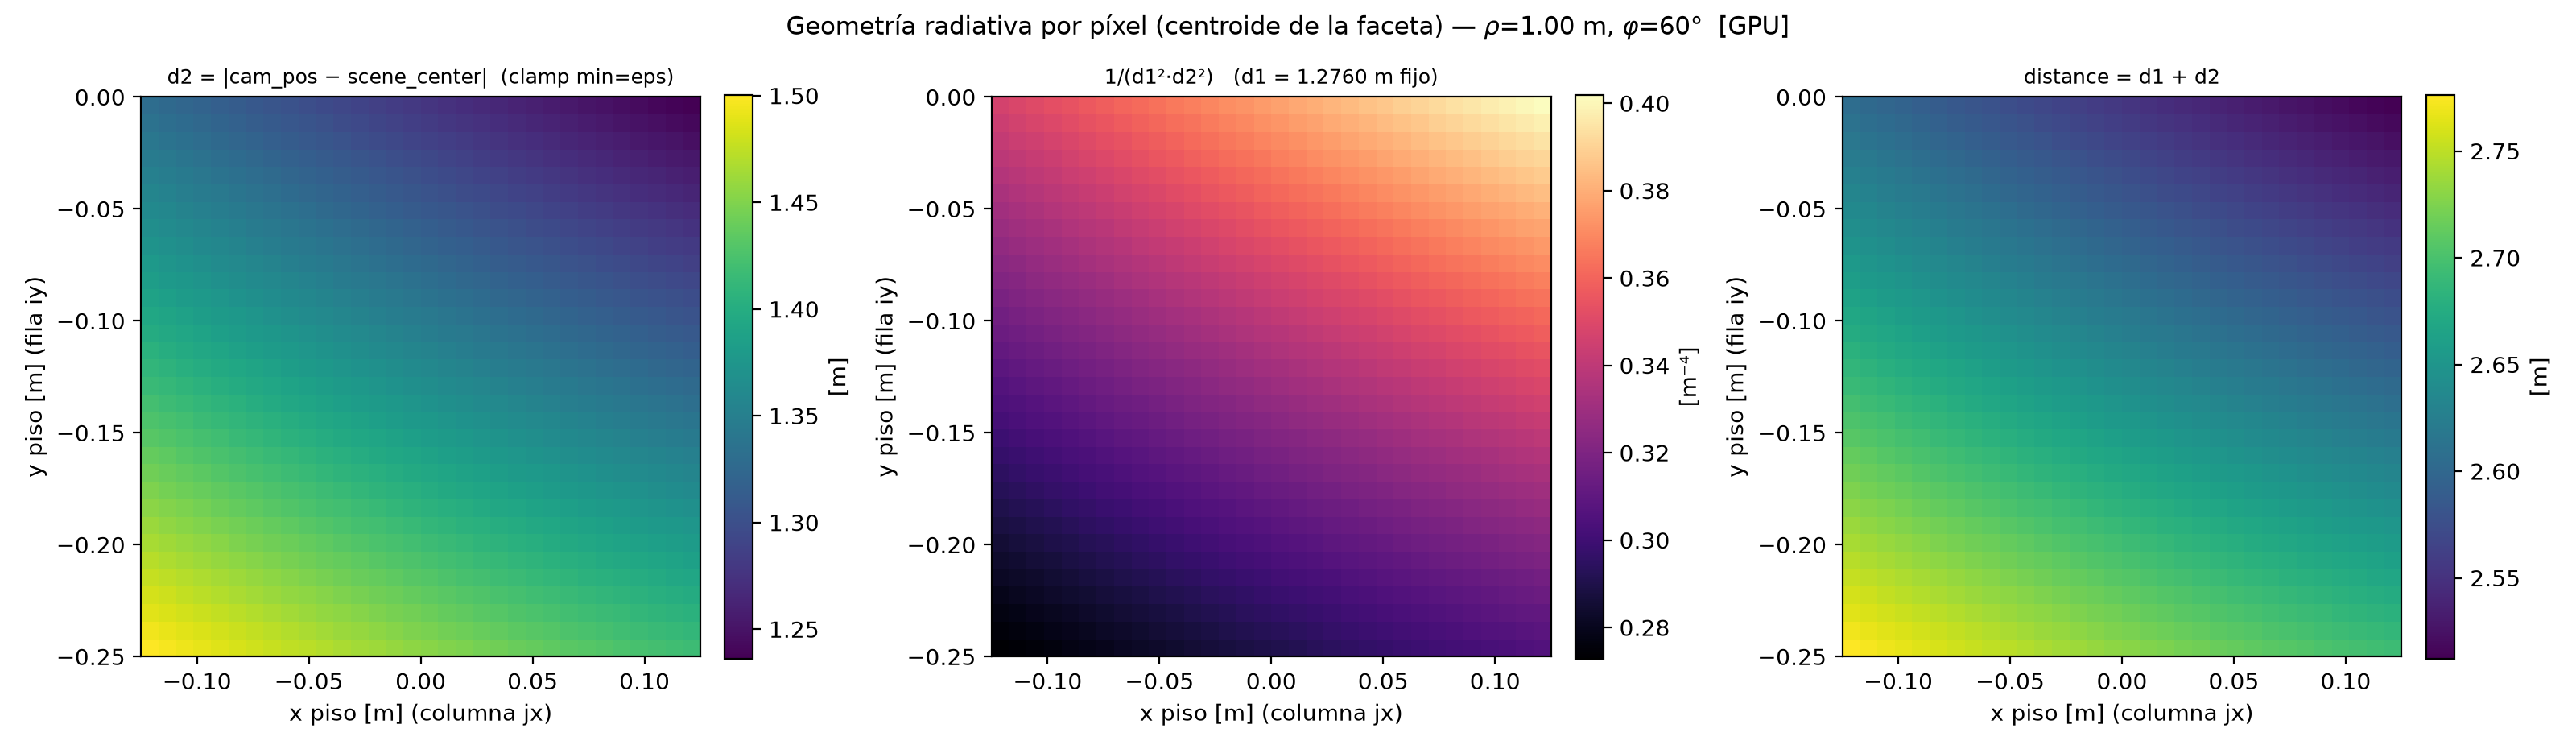
\includegraphics[width=\textwidth]{crb_sim_components_gpu_geometry.png}}{%
  \fbox{\parbox{0.9\textwidth}{\centering\vspace{2em}(figura no
  disponible)\vspace{2em}}}}
\caption{Geometría radiativa por píxel para el centroide de la faceta en
$(\rho,\varphi)=(1\,\text{m},60^\circ)$. Izquierda: $d_2$, que varía solo entre
$1.24$ y $1.50\,$m sobre todo el FOV. Centro: la atenuación
$1/(d_1^2d_2^2)$ con $d_1=1.276\,$m fijo. Derecha: el camino total $d_1+d_2$,
que es lo que se cuantiza en \emph{bins}. Generada por
\code{plot\_simulator\_components.py --backend gpu}.}
\label{fig:geometria}
\end{figure}

%-----------------------------------------------------------------------
\subsection{Los cuatro cosenos}
\label{sec:cosenos}

Cada reflexión difusa obedece la ley de Lambert: la potencia que una superficie
emite o recibe en una dirección se reduce por el coseno del ángulo entre esa
dirección y la normal, porque lo que cuenta es el \emph{área proyectada}
perpendicular al haz. En un trayecto de dos rebotes hay cuatro eventos de este
tipo --- una emisión y una incidencia en cada una de las dos superficies --- y
el código los calcula exactamente así:

\begin{equation}
\label{eq:dots}
\begin{aligned}
\text{\code{dot3}} &= \max\Bigl(0,\ \Bigl\langle \vect n_\ell,\
   \tfrac{\vect c_t-\vect p_\ell}{d_1}\Bigr\rangle\Bigr)
   &&\text{emisión en el punto iluminado del suelo,}\\[1mm]
\text{\code{dot1}} &= \max\Bigl(0,\ \Bigl\langle \vect n_t,\
   \tfrac{\vect p_\ell-\vect c_t}{d_1}\Bigr\rangle\Bigr)
   &&\text{incidencia en la faceta,}\\[1mm]
\text{\code{dot2}} &= \max\Bigl(0,\ \Bigl\langle \vect n_t,\
   \tfrac{\vect q_p-\vect c_t}{d_2}\Bigr\rangle\Bigr)
   &&\text{emisión desde la faceta,}\\[1mm]
\text{\code{dot4}} &= \max\Bigl(0,\ \Bigl\langle \vect n_{\text{piso}},\
   \tfrac{\vect c_t-\vect q_p}{d_2}\Bigr\rangle\Bigr)
   &&\text{incidencia en el parche de suelo,}
\end{aligned}
\end{equation}
%
con $\vect n_{\text{piso}}=(0,0,1)$ (\code{floor\_normal}).

\paragraph{Correspondencia exacta con el código, incluidos los signos.}
Merece la pena seguirlos uno a uno, porque los signos son fáciles de confundir.
El código define \code{lps = laser\_pos - centers}, es decir
$\vect p_\ell-\vect c_t$, y \code{fovsp = cam\_pos - centers}, es decir
$\vect q_p-\vect c_t$. Entonces:
%
\begin{itemize}[leftmargin=*]
  \item \code{dot1 = clamp(sum(normals * (lps/d1)))}: usa
        $+\vect{\text{lps}}$, o sea la dirección \emph{de la faceta hacia el
        láser}. Correcto para una incidencia: se mide el ángulo entre la normal
        de la faceta y la dirección de donde viene la luz.
  \item \code{dot3 = clamp(sum(laser\_normal * (-lps/d1)))}: usa
        $-\vect{\text{lps}} = \vect c_t-\vect p_\ell$, la dirección
        \emph{del láser hacia la faceta}. Correcto para una emisión: se mide el
        ángulo entre la normal del emisor y la dirección de salida.
  \item \code{dot2 = clamp(sum(normals * (fovsp/d2)))}: usa
        $+\vect{\text{fovsp}}$, dirección \emph{de la faceta hacia el píxel}:
        emisión desde la faceta.
  \item \code{dot4 = clamp(sum(floor\_normal * (-fovsp/d2)))}: usa
        $-\vect{\text{fovsp}} = \vect c_t - \vect q_p$, dirección \emph{del
        píxel hacia la faceta}: incidencia sobre el suelo.
\end{itemize}
%
El patrón es consistente: en las \emph{emisiones} el vector apunta
\emph{alejándose} del emisor, y en las \emph{incidencias} apunta \emph{hacia} la
fuente. Los dos que usan el signo negativo son precisamente los dos que se
miden contra una normal que no es la de la faceta.

\paragraph{Por qué el \code{clamp}.}
$\max(0,\cdot)$ implementa el hecho físico de que \textbf{una cara no irradia
hacia atrás ni recibe luz por detrás}. Si $\langle\vect n,\vect u\rangle<0$, la
dirección $\vect u$ está en el hemisferio opuesto a la cara y la contribución
debe ser cero, no negativa. Sin el \code{clamp} los triángulos orientados al
revés restarían energía y podrían producir intensidades negativas, que además
romperían el modelo de Poisson de la sección~\ref{sec:estadistico} (una tasa no
puede ser negativa).

En la pose de la figura~\ref{fig:cosenos} el \code{clamp} está \textbf{inactivo}
(los mínimos sin recortar son $0.762$ para \code{dot2} y $0.528$ para
\code{dot4}, ambos positivos): con la faceta mirando al origen y el FOV
pequeño, ningún píxel cae detrás de la faceta. El \code{clamp} es una guarda que
solo se activa en poses extremas, pero su presencia es la razón por la que el
\emph{forward} es no diferenciable en un conjunto de medida no nula de
configuraciones (sección~\ref{sec:fd}).

\begin{figure}[htbp]
\centering
\IfFileExists{../plots/crb_sim_components_gpu_cosines.png}{%
  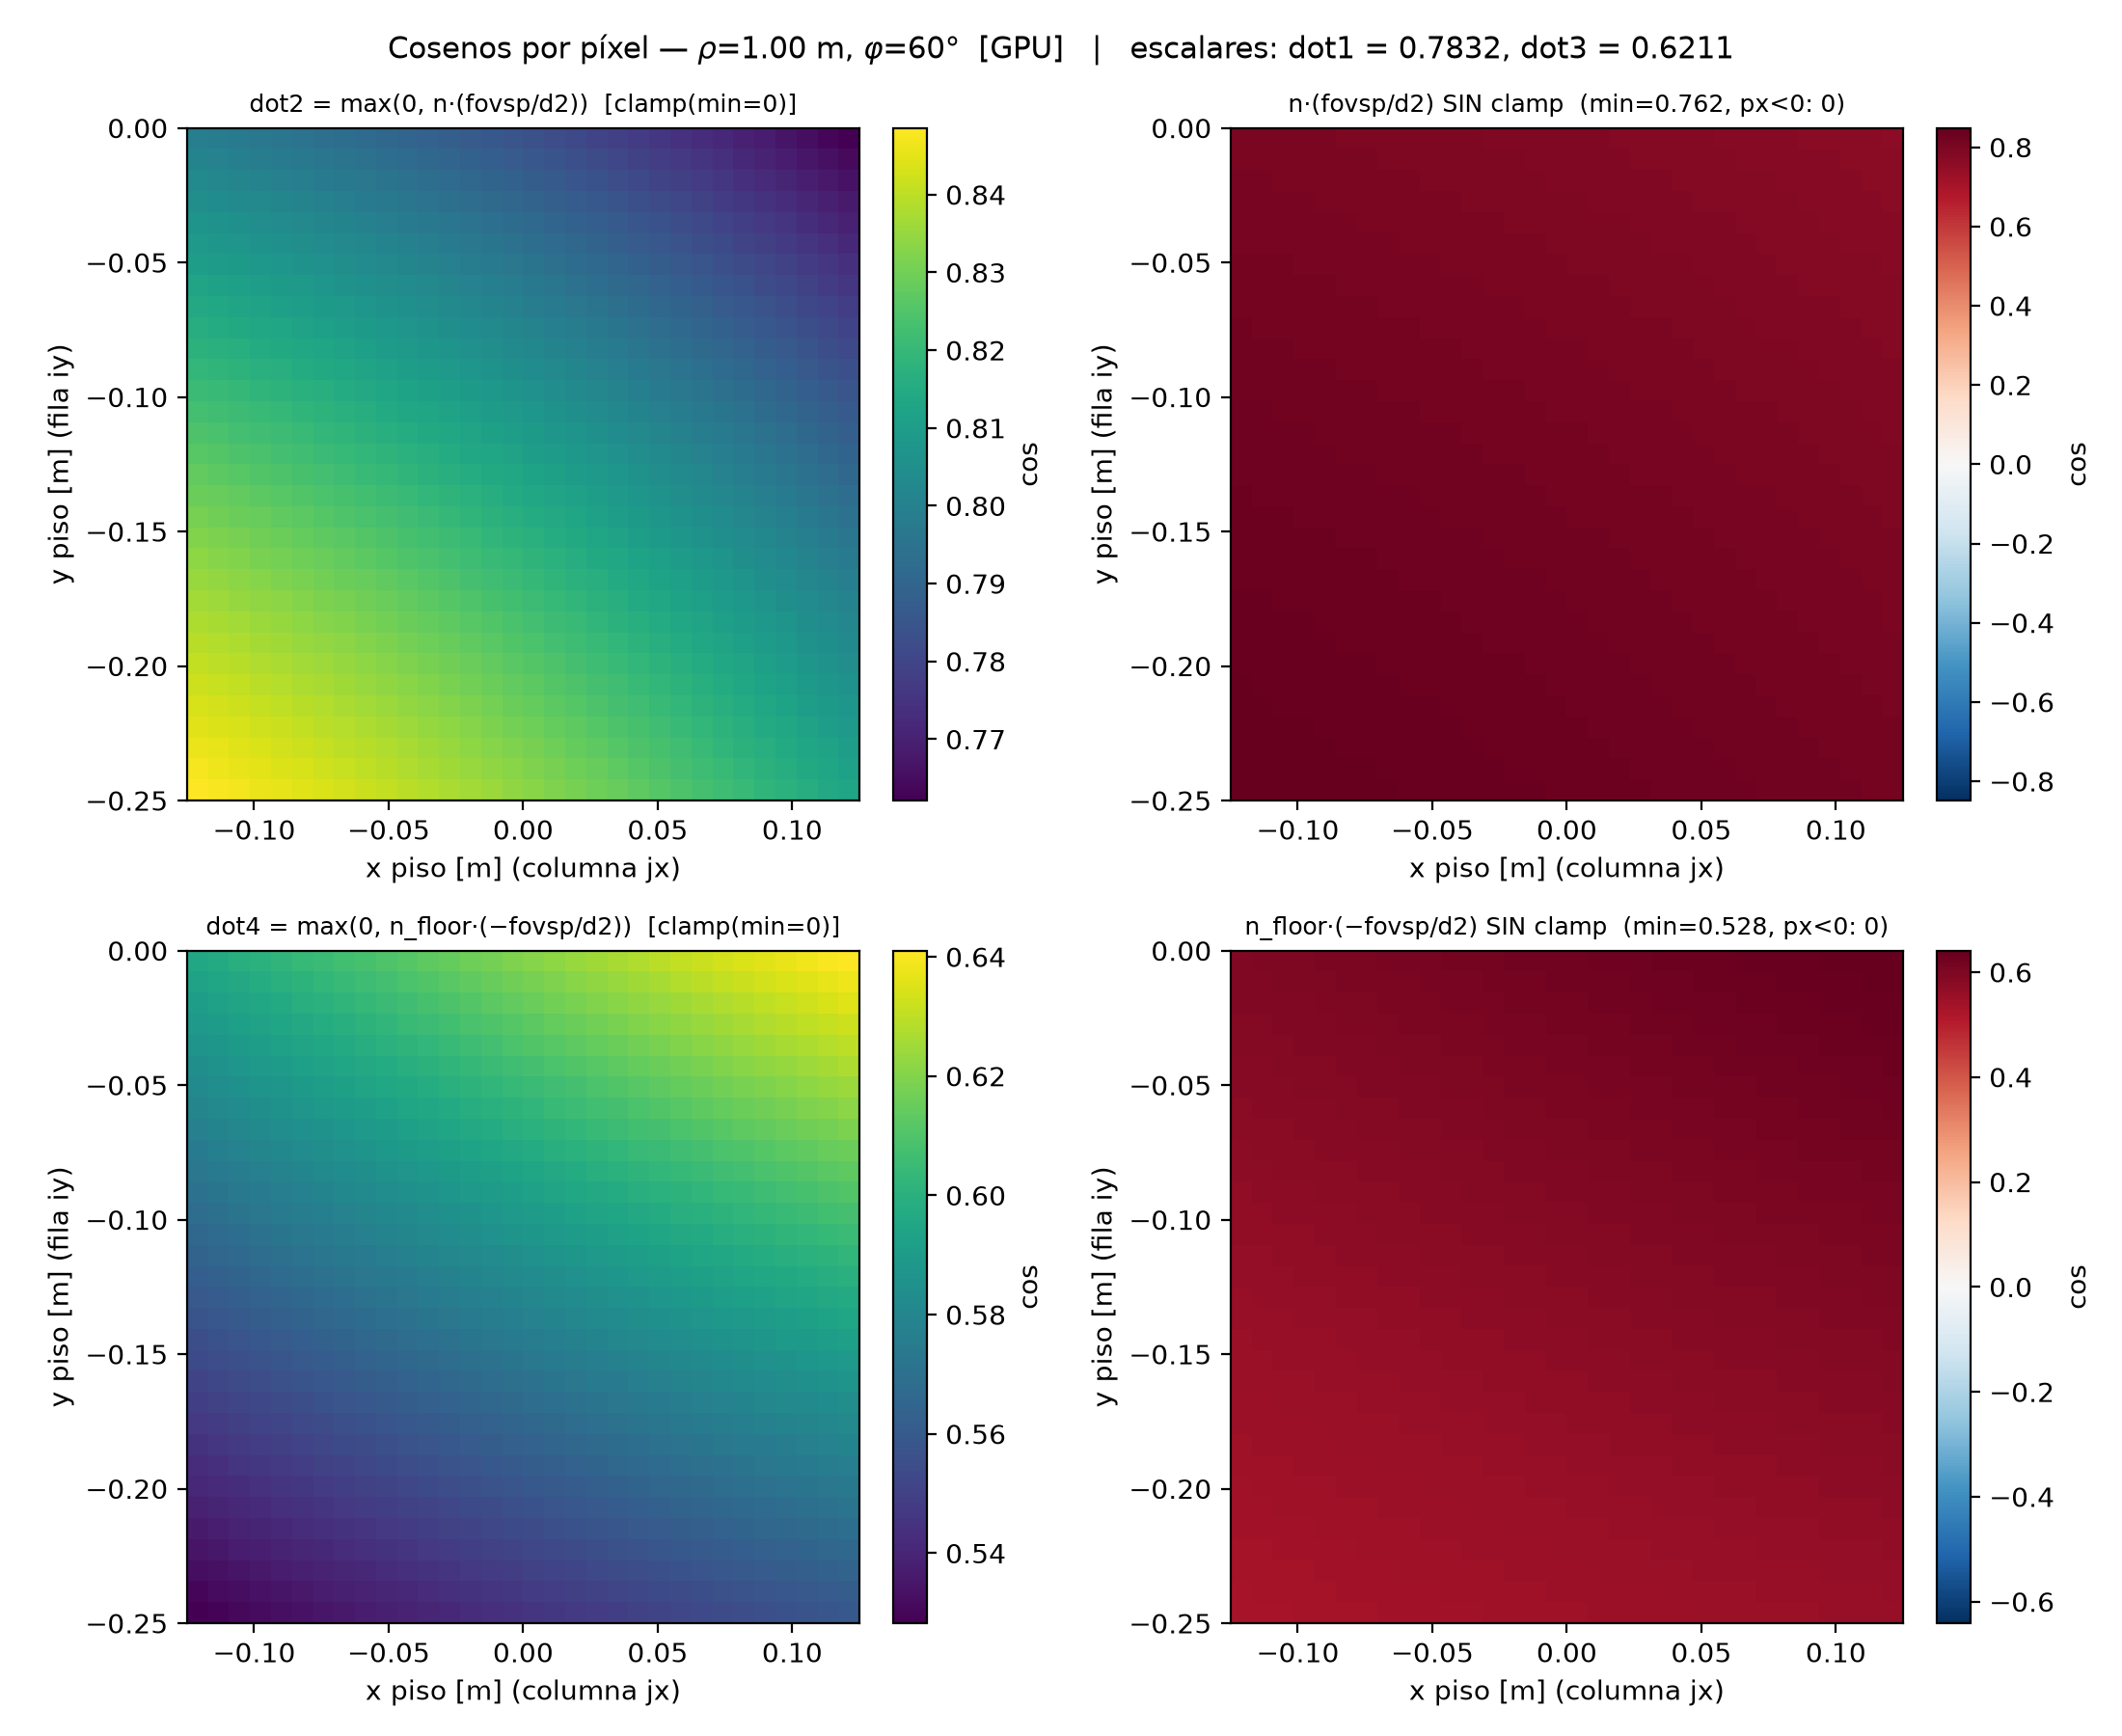
\includegraphics[width=0.94\textwidth]{crb_sim_components_gpu_cosines.png}}{%
  \fbox{\parbox{0.9\textwidth}{\centering\vspace{2em}(figura no
  disponible)\vspace{2em}}}}
\caption{Los cosenos dependientes del píxel, \code{dot2} y \code{dot4}, con y
sin \code{clamp}, para $(\rho,\varphi)=(1\,\text{m},60^\circ)$. Los escalares
que solo dependen del triángulo valen \code{dot1}$=0.7832$ y
\code{dot3}$=0.6211$. Las columnas de la derecha muestran que en esta pose no
hay ningún píxel con coseno negativo: el \code{clamp} no actúa.}
\label{fig:cosenos}
\end{figure}

%-----------------------------------------------------------------------
\subsection{La atenuación \texorpdfstring{$1/(4\pi^2 d_1^2 d_2^2)$}{1/(4 pi^2 d1^2 d2^2)}}
\label{sec:atenuacion}

El código escribe la intensidad como
%
\begin{equation}
\label{eq:intensity}
\boxed{\ 
I_{t,p} = \frac{I_{\text{láser}}\; A_t\;
   \text{\code{dot1}}\cdot\text{\code{dot2}}\cdot\text{\code{dot3}}\cdot\text{\code{dot4}}}
   {4\pi^2\; d_1^2\; d_2^2}\ }
\end{equation}
%
es decir, en el código,
%
\begin{center}
\code{intensity = laser\_intensity * area * (dot1*dot2*dot3*dot4)}\\
\code{\qquad / (fourpi * d1s * d2s)} ,
\end{center}
%
con \code{fourpi = 4.0 * torch.pi * torch.pi}.

\paragraph{Los dos $1/d^2$.}
Cada tramo de propagación libre reparte la energía emitida sobre una superficie
que crece como el cuadrado de la distancia, así que la irradiancia que llega cae
como $1/d^2$. Hay dos tramos ($d_1$ y $d_2$) y por tanto dos factores. Es
importante notar que el código usa $d_1^2$ y $d_2^2$ \textbf{sin raíz}
(\code{d1s} y \code{d2s} son las normas al cuadrado), lo que evita dos raíces
cuadradas por elemento; las raíces $d_1$ y $d_2$ se calculan aparte solo para
normalizar los vectores de los cosenos y para el tiempo de vuelo.

\paragraph{La constante $4\pi^2$.}
Cada reflexión difusa reparte la potencia incidente sobre un hemisferio
completo, cuyo ángulo sólido es $2\pi\,$sr; normalizar para que la energía se
conserve introduce un factor $1/(2\pi)$ por reflexión. Como aquí hay
\textbf{dos} eventos de emisión difusa (el punto iluminado del suelo y la
faceta),
%
\begin{equation}
\label{eq:4pi2}
(2\pi)^2 = 4\pi^2 \approx 39.478 .
\end{equation}
%
Esta lectura es autoconsistente con la del \emph{writeup} de referencia, que usa
$8\pi^3=(2\pi)^3$: allí hay \textbf{tres} emisiones difusas porque se modela
también el tramo suelo$\to$cámara como una reflexión. Aquí ese tramo no es una
reflexión (el SPAD observa el parche directamente, sección~\ref{sec:distancias}),
de ahí que sobre un factor $2\pi$. La regla mnemotécnica es
$(2\pi)^{\#\text{emisiones difusas}}$.

\begin{salvedad}[La constante global \emph{sí} afecta al CRB]
\label{sal:constante}
Podría parecer que un factor multiplicativo global en $\vect y$ es irrelevante
porque \enquote{se cancela}. No es así. Con ruido de Poisson la varianza
\emph{es} la media, de modo que al escalar $\vect y\mapsto\alpha\vect y$ con el
fondo $b$ fijo, la información de Fisher \eqref{eq:fisher} no escala de forma
trivial y el CRB cambia. En el régimen dominado por señal ($y\gg b$) se tiene
$\matr I\propto\alpha$ y por tanto $\sigma\propto\alpha^{-1/2}$: cuadruplicar la
potencia del láser reduce las $\sigma$ a la mitad. Las constantes radiométricas
y \code{laser\_intensity}$=1000$ son, por tanto, parte del resultado y no
adornos.
\end{salvedad}

%-----------------------------------------------------------------------
\subsection{Área del triángulo e intensidad del láser}
\label{sec:area}

El factor $A_t$ de \eqref{eq:intensity} es el peso de la cuadratura
\eqref{eq:cuadratura}: la contribución de un triángulo es proporcional a su
elemento de superficie. El código lo calcula con la mitad de la norma del
producto vectorial de dos aristas,
%
\begin{equation}
A_t = \tfrac12\bigl\lVert (\vect v_2-\vect v_1)\times(\vect v_3-\vect v_1)\bigr\rVert ,
\end{equation}
%
que es la fórmula exacta del área de un triángulo en $\mathbb R^3$
(\code{areas = 0.5 * norm(cross(...))}). Sumando sobre los $32\,768$ triángulos
se recupera el área total de la faceta, $0.79251\,\text{m}^2 = 0.5\times1.585$,
lo que confirma que la densificación conserva la geometría.

El factor $I_{\text{láser}}=$\code{laser\_intensity}$=1000$ fija la escala
absoluta. Su papel es el de la salvedad~\ref{sal:constante}: convierte el
resultado geométrico en un número de cuentas esperadas.

%-----------------------------------------------------------------------
\subsection{Oclusión: derivación de \texorpdfstring{$x_{\text{int}}$}{x\_int}}
\label{sec:oclusion}

Este es el paso menos evidente del código y el que aporta casi toda la
información angular, así que conviene derivarlo con cuidado.

\paragraph{El problema.}
Un triángulo de la faceta (en $y>0$) puede enviar luz a un píxel del suelo (en
$y<0$) solo si el segmento que los une pasa por el hueco de la esquina. La
arista ocluyente está sobre $y=0$ y tapa $x<0$. Proyectado sobre el plano
horizontal, el segmento cruza la recta $y=0$ exactamente una vez, y la pregunta
es \emph{en qué $x$}.

\paragraph{La derivación.}
Sean $(c_x,c_y)$ la proyección horizontal del centroide del triángulo y
$(q_x,q_y)$ la del píxel. La recta que los une, en forma $y=mx+b$, tiene
pendiente y ordenada
%
\begin{equation}
\label{eq:mb}
m = \frac{c_y-q_y}{c_x-q_x},
\qquad
b = c_y - m\,c_x ,
\end{equation}
%
que es literalmente lo que hace el código:
%
\begin{center}
\code{denom = cx - cam\_x};\quad
\code{m = (cy - cam\_y) / denom};\quad
\code{b = cy - m * cx} .
\end{center}
%
El cruce con $y=0$ se obtiene resolviendo $0=m\,x+b$:
%
\begin{equation}
\label{eq:xint}
\boxed{\ x_{\text{int}} = -\frac{b}{m}\ }
\qquad\text{(\code{xint = -b / m})}.
\end{equation}

\paragraph{Por qué $x_{\text{int}}>0$ es el test correcto.}
Como el centroide está en $y>0$ y el píxel en $y<0$, el punto de cruce
$(x_{\text{int}},0)$ está \emph{dentro} del segmento, no en su prolongación. Por
tanto:
%
\begin{itemize}[leftmargin=*]
  \item $x_{\text{int}}>0$: el segmento atraviesa $y=0$ del lado abierto de la
        esquina, luego el camino está libre y el par (triángulo, píxel) es
        visible;
  \item $x_{\text{int}}<0$: el segmento intentaría atravesar la pared, luego el
        camino está bloqueado.
\end{itemize}
%
El código lo escribe como
\code{noc = isfinite(xint) \& (xint > 0)} (\emph{no occlusion}). Es un modelo de
oclusión \textbf{de medio plano}: la pared se supone infinita en $x<0$ y de
altura infinita, así que basta el test horizontal. Esa es la simplificación que
hace que la oclusión salga gratis, sin trazar rayos contra ninguna geometría.

\paragraph{Las guardas numéricas de la versión GPU.}
Si el centroide y el píxel tienen la misma $x$, la recta es vertical y $m$
diverge. El código lo evita con
%
\begin{center}
\code{valid\_denom = abs(denom) > eps};\quad
\code{m = where(valid\_denom, (cy-cam\_y)/denom, nan)},
\end{center}
%
con \code{eps}$=10^{-12}$, y después el \code{isfinite(xint)} descarta esos
casos. Poner \code{nan} y filtrar es preferible a poner un número grande, porque
un $m$ enorme daría un $x_{\text{int}}$ minúsculo de signo arbitrario, es decir,
una decisión de visibilidad esencialmente aleatoria. En la pose verificada
ningún elemento cae en este caso ($0$ máscaras activas, $0$ $x_{\text{int}}$ no
finitos), pero la guarda evita un fallo silencioso.

\begin{salvedad}[El test es por centroide: no hay visibilidad parcial]
\label{sal:centroide}
La visibilidad se decide por el \emph{centroide} de cada triángulo: un triángulo
está entero visible o entero oculto. La frontera real de la sombra corta
triángulos por la mitad, y ese corte no se modela. El error que esto introduce
es de orden \enquote{un triángulo} en la frontera, y es precisamente por eso que
la densificación a $32\,768$ triángulos (observación~\ref{obs:ntri}) importa:
cuanto más finos los triángulos, mejor se aproxima la frontera. Tampoco hay
supermuestreo dentro del píxel; el simulador antiguo tenía un parámetro
\code{subpixel\_dim} que el nuevo no usa.
\end{salvedad}

La figura~\ref{fig:oclusion} muestra el campo $x_{\text{int}}$ sobre la grilla y
la máscara resultante: para el centroide de la faceta en
$(1\,\text{m},60^\circ)$, $802$ de los $1024$ píxeles ven la faceta, y la
frontera $x_{\text{int}}=0$ es una recta en el plano del suelo.

\begin{figure}[htbp]
\centering
\IfFileExists{../plots/crb_sim_components_gpu_occlusion.png}{%
  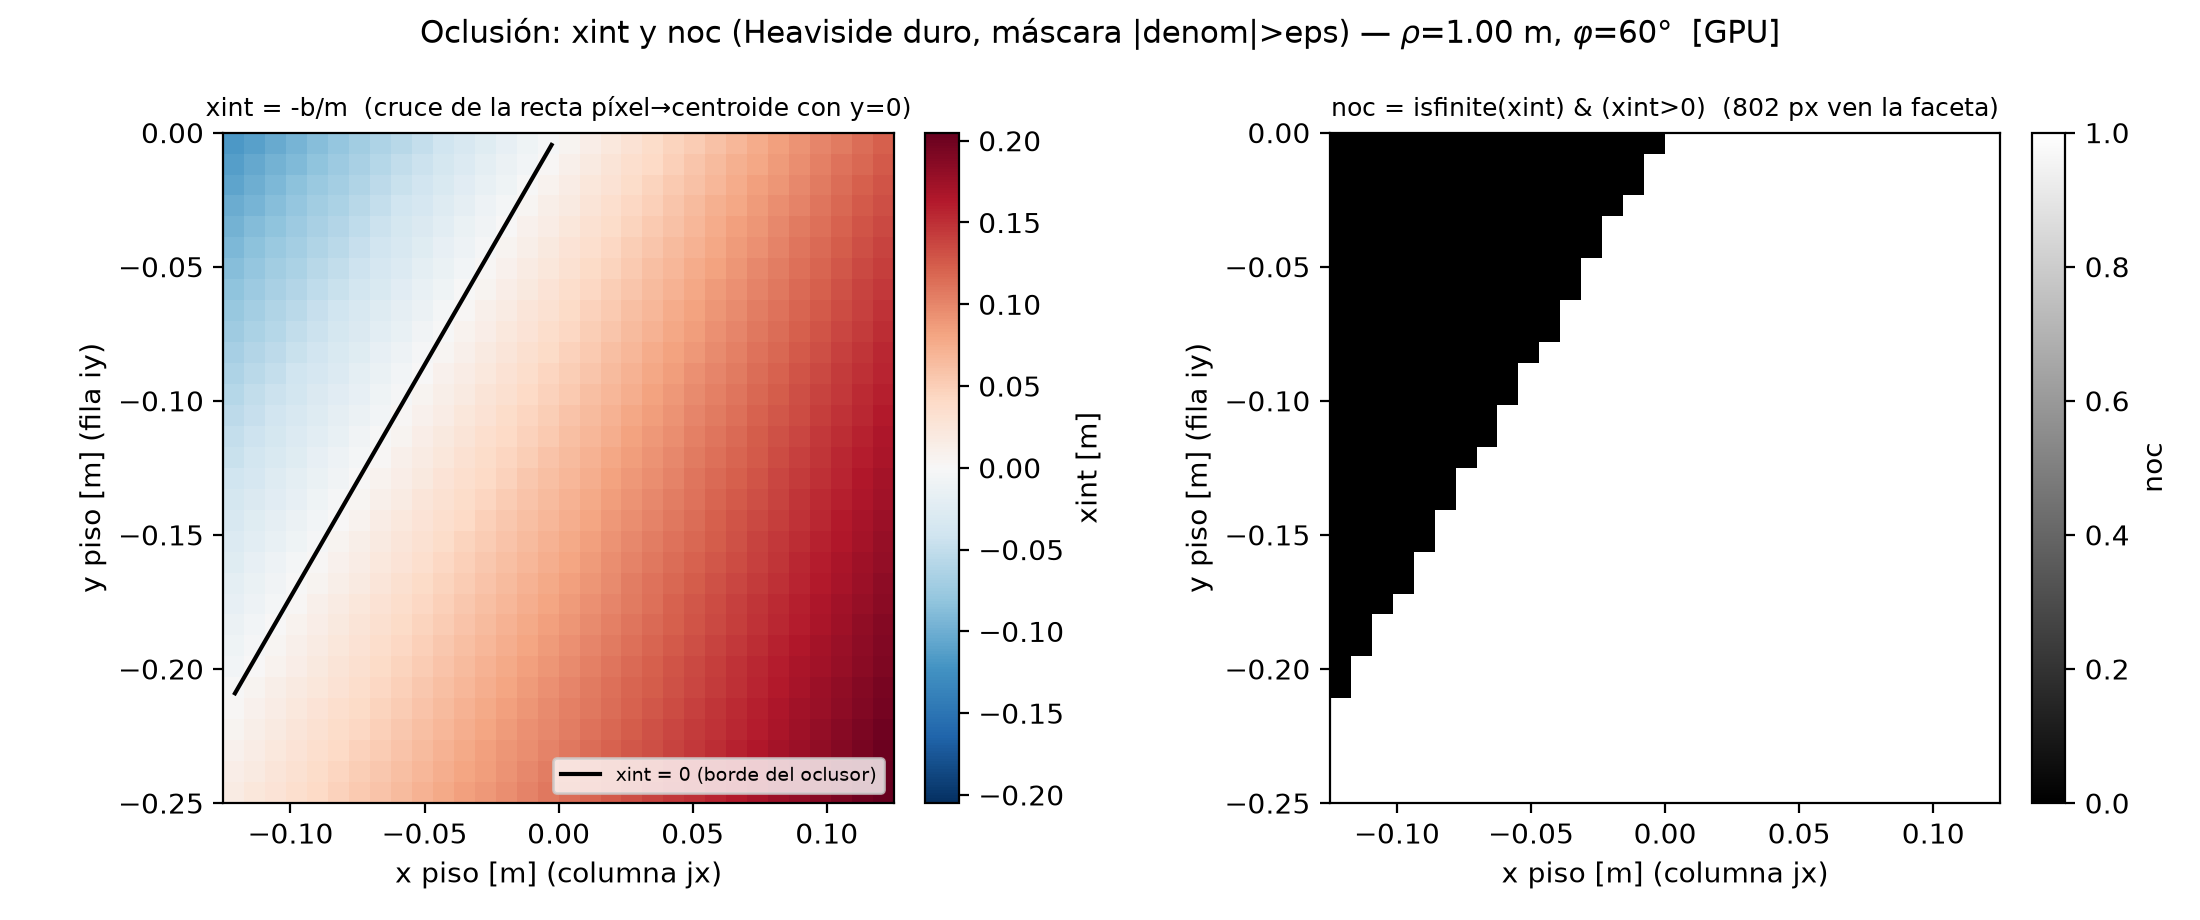
\includegraphics[width=\textwidth]{crb_sim_components_gpu_occlusion.png}}{%
  \fbox{\parbox{0.9\textwidth}{\centering\vspace{2em}(figura no
  disponible)\vspace{2em}}}}
\caption{Izquierda: $x_{\text{int}}=-b/m$ por píxel, con la línea negra marcando
$x_{\text{int}}=0$ (el borde de la sombra del oclusor). Derecha: la máscara
booleana \code{noc}, escalonada con el paso de la grilla porque la decisión es
por píxel y por centroide. Esta discontinuidad es la fuente de la información
angular \emph{y} el principal obstáculo a la diferenciación.}
\label{fig:oclusion}
\end{figure}

%-----------------------------------------------------------------------
\subsection{Cuantización temporal y depósito}
\label{sec:binning}

\paragraph{Tiempo de vuelo y \emph{bin}.}
El tiempo que tarda la luz en recorrer el camino de dos rebotes es
$t_0=(d_1+d_2)/c$, y el \emph{bin} en que el SPAD lo registra es
%
\begin{equation}
\label{eq:bin}
j(t,p) = \Bigl\lceil \frac{d_1(t)+d_2(t,p)}{c\,\Delta t}\Bigr\rceil
\qquad\text{(\code{arrival\_bin = ceil((d1+d2)/(C*bin\_size))})}.
\end{equation}
%
El $\lceil\cdot\rceil$ es el modelo del contador: un SPAD con \emph{binning} de
anchura $\Delta t$ no informa del instante exacto de llegada, sino del intervalo
$[\,(j-1)\Delta t,\ j\Delta t\,)$ en que cayó. Toda la masa del triángulo se
deposita íntegra en ese \emph{bin}; no se reparte entre \emph{bins} vecinos. El
código valida además que el índice caiga en rango:
\code{valid = noc \& (arrival\_bin > 0) \& (arrival\_bin <= num\_time\_bins)}.

\paragraph{Cuántos \emph{bins} hay: \code{num\_time\_bins}.}
El eje temporal se dimensiona a partir del camino más largo posible en la
escena:
%
\begin{equation}
\label{eq:T}
T = \Bigl\lceil \frac{d_{\max}}{c\,\Delta t}\times 1.2\Bigr\rceil,
\qquad
d_{\max} = \lVert \vect p_{\text{esc}}\rVert +
           \lVert \vect p_{\text{spad}}-\vect p_{\text{esc}}\rVert ,
\end{equation}
%
con $\vect p_{\text{esc}}=(x_{\max},y_{\max},z_{\max})=(1.5,3,3)$ la esquina más
lejana del volumen de escena y
$\vect p_{\text{spad}}=(-\text{FOV}/2,-\text{FOV},0)=(-0.125,-0.25,0)$ la del
parche observado. Numéricamente $d_{\max}=9.2120\,$m y
%
\[
T = \bigl\lceil 9.2120/c/(3.9\cdot10^{-10})\times1.2 \bigr\rceil = 95 .
\]
%
El margen de $1.2$ es un colchón del 20\%: garantiza que ningún camino real
se salga del cubo, aun con objetos colocados en los límites del volumen. Si
faltara, los \emph{bins} tardíos se descartarían por la máscara \code{valid} y
se perdería energía en silencio.

\paragraph{Depósito disperso.}
El código no construye un tensor $T_\triangle\times P\times T$ (sería enorme),
sino que aplana la salida y suma con un \emph{scatter-add}:
%
\begin{equation}
\label{eq:coord}
\texttt{coord} = (j-1)\cdot P + \texttt{pixel\_linear}[p],
\qquad
\texttt{y\_meas\_vec.index\_add\_(0, coord, intensity)} .
\end{equation}
%
El uso de \code{index\_add\_} en lugar de una asignación es \emph{obligatorio}:
muchísimos pares (triángulo, píxel) comparten el mismo \code{coord}, y lo que se
quiere es la \textbf{suma} de sus contribuciones, que es exactamente la
cuadratura \eqref{eq:cuadratura}. Una asignación se quedaría con una
contribución arbitraria.

\paragraph{El índice \code{pixel\_linear} y el \code{reshape} en orden Fortran.}
Este par de líneas es el que más confunde, así que lo desmenuzamos. Los centros
de píxel se generan con \code{meshgrid(pixel\_y, pixel\_x, indexing="ij")} y se
aplanan en orden C, de modo que el píxel $k$ tiene coordenadas
$(x_{j},y_{i})$ con $i=k\;\mathrm{div}\;N$ y $j=k\bmod N$. El código define
%
\begin{equation}
\texttt{pixel\_linear}[k] = \underbrace{(k\bmod N)}_{j}\cdot N +
                            \underbrace{(k\;\mathrm{div}\;N)}_{i}
                          = jN+i ,
\end{equation}
%
es decir, \textbf{transpone} el índice. Al final se hace
\code{reshape((N,N,T), order="F")}, y en orden Fortran el índice plano $f$
corresponde a $(a,b,c)$ con $f=a+Nb+N^2c$. Sustituyendo \eqref{eq:coord}:
$c=j-1$ (el \emph{bin}, base cero) y $a+Nb=jN+i$, de donde $a=i$ y $b=j$. Por
tanto
%
\begin{equation}
\label{eq:ejes}
\boxed{\ \vect y[\,a,b,c\,] \ \text{con}\
a = \text{índice de píxel en } y,\quad
b = \text{índice de píxel en } x,\quad
c = j-1 .\ }
\end{equation}
%
La transposición de \code{pixel\_linear} y el \code{order="F"} se
\textbf{cancelan} entre sí y dejan el orden de ejes
(\code{y\_pixels}, \code{x\_pixels}, \code{time\_bins}) que el propio código
declara en los atributos del HDF5. Verificado exhaustivamente con una malla de
prueba $4\times4\times3$.

\paragraph{El \code{roll} de orientación.}
Por último, \code{simulation} aplica
%
\begin{equation}
\label{eq:roll}
\vect y \longleftarrow \texttt{np.roll}(\vect y,\ \text{shift}=1,\ \text{axis}=1)
\qquad\text{(\code{orient\_transient\_measurement})} ,
\end{equation}
%
una permutación cíclica de una posición a lo largo del eje de píxeles en $x$.
Es una corrección de orientación heredada, y comprobadamente activa: la salida
real difiere de la no rotada. Su efecto visible es que la columna $j=N-1$ pasa a
ocupar $j=0$, lo que en la figura~\ref{fig:transitorio} se aprecia como una
columna \enquote{fuera de lugar} en el borde izquierdo. Ahora bien:

\begin{prop}[El \code{roll} no altera el CRB]
\label{prop:roll}
Sea $\pi$ cualquier permutación de los índices de medición y sea
$\vect g^\pi_q=\vect g_{\pi(q)}$. Entonces la información de Fisher de
\eqref{eq:fisher} cumple $\matr I[\vect g^\pi]=\matr I[\vect g]$, y por tanto el
CRB, las $\sigma$ y las elipses son idénticos.
\end{prop}

\begin{proof}
$\matr I_{mk}=\sum_q \frac{1}{g_q}\partial_m g_q\,\partial_k g_q$ es una suma
sobre \emph{todos} los índices $q$. Como $\pi$ es una biyección del conjunto de
índices sobre sí mismo, reordenar los sumandos no cambia la suma. Además el
fondo $b$ es constante, luego $\vect g^\pi=\pi(\vect y)+b=\pi(\vect y+b)$ y la
permutación conmuta con la suma del fondo.
\end{proof}

Comprobado numéricamente: recalculando el CRB con el \code{roll} deshecho, la
diferencia relativa máxima en $\matr I$ es $1.3\cdot10^{-16}$ en
$(1\,\text{m},90^\circ)$ y $1.2\cdot10^{-15}$ en $(0.5\,\text{m},30^\circ)$, con
$\Delta\sigma_\rho=0$ exactamente. Es decir: el \code{roll} importa si se van a
\emph{mirar} las imágenes o reconstruir la escena, y es irrelevante para todo lo
que sigue en estas notas.

\paragraph{Cuán cuantizado está el rango.}
Aquí hay que distinguir dos cosas que a menudo se confunden.

\emph{Para un punto fijo de la faceta}, el \emph{bin} de llegada apenas varía
sobre la imagen: en la figura~\ref{fig:binning}, el centroide produce solo
\textbf{tres} valores enteros distintos ($22$, $23$, $24$) en los $1024$
píxeles, porque $d_2$ recorre menos de $26\,$cm sobre todo el FOV. El corte 1D
de la derecha muestra la escalera del $\lceil\cdot\rceil$ frente a la recta
continua: mesetas largas separadas por saltos.

\emph{Para la faceta completa}, en cambio, el transitorio de un solo píxel ocupa
del orden de $15$ a $21$ \emph{bins}, porque los $32\,768$ triángulos se
reparten a lo largo de $1.585\,$m de altura y sus caminos $d_1+d_2$ difieren
mucho. Medido sobre la salida real:
%
\begin{center}
\small
\begin{tabular}{@{}llrrr@{}}
\toprule
$\rho$ [m] & $\varphi$ [$^\circ$] & \emph{bins} con señal
& píxeles iluminados & \emph{bins} por píxel (medio) \\
\midrule
0.5 & 30  & 7--29  & 1016/1024 & 20.9 \\
1.0 & 60  & 16--33 & 888/1024  & 15.9 \\
1.0 & 90  & 17--33 & 640/1024  & 15.7 \\
1.5 & 150 & 25--38 & 105/1024  & 12.7 \\
\bottomrule
\end{tabular}
\end{center}
%
Las dos afirmaciones son compatibles y ambas serán importantes: la primera
explica por qué la derivada respecto de $\rho$ es problemática
(sección~\ref{sec:fd}), y la segunda por qué a pesar de todo funciona.

\begin{figure}[htbp]
\centering
\IfFileExists{../plots/crb_sim_components_gpu_binning.png}{%
  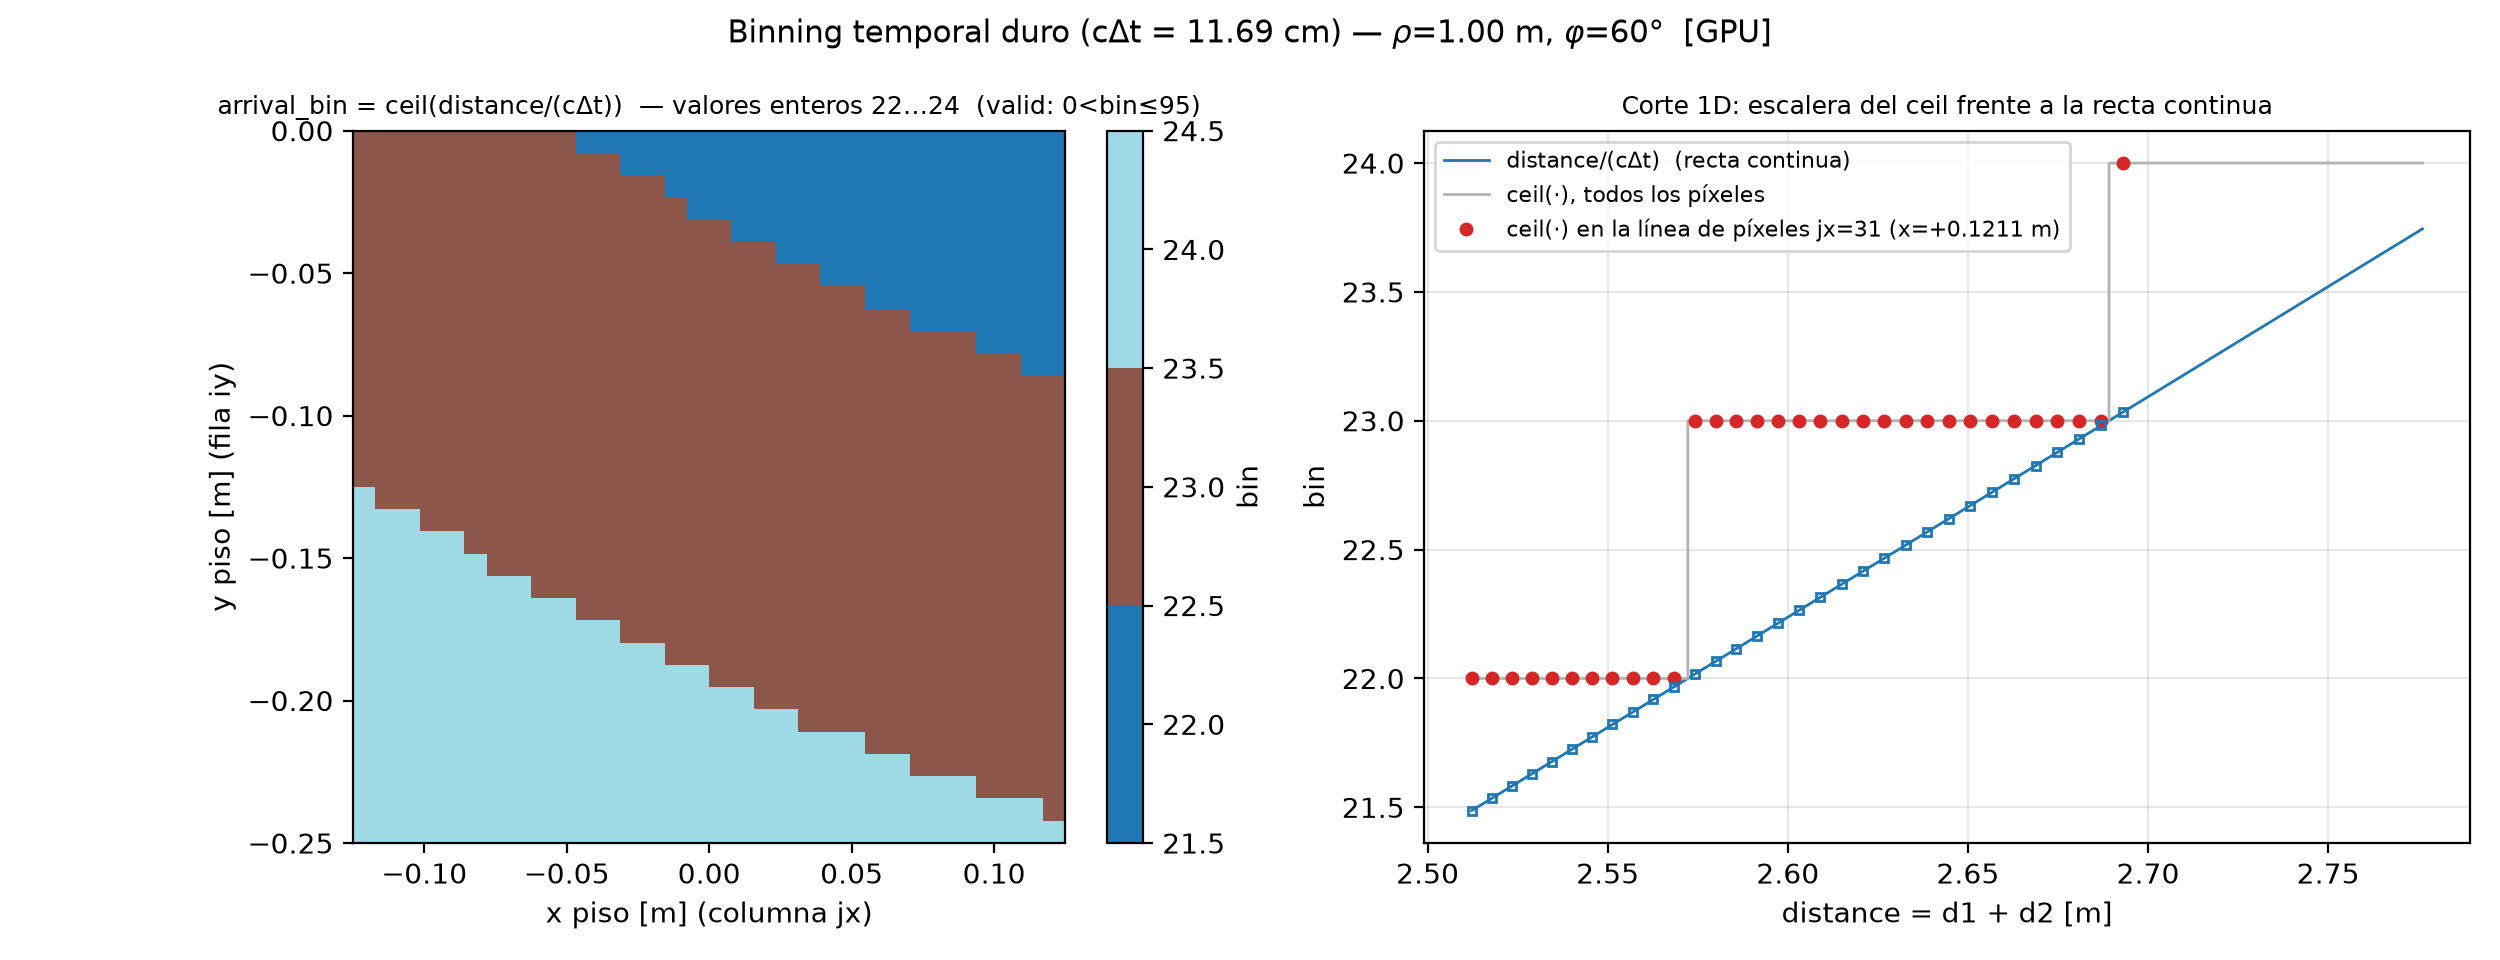
\includegraphics[width=\textwidth]{crb_sim_components_gpu_binning.png}}{%
  \fbox{\parbox{0.9\textwidth}{\centering\vspace{2em}(figura no
  disponible)\vspace{2em}}}}
\caption{Cuantización temporal para el centroide de la faceta. Izquierda: el
\emph{bin} de llegada toma solo los valores $22,23,24$ sobre la grilla entera.
Derecha: la escalera del $\lceil\cdot\rceil$ contra la recta continua
$(d_1+d_2)/(c\Delta t)$, sobre la fila de píxeles $j=31$.}
\label{fig:binning}
\end{figure}

%-----------------------------------------------------------------------
\subsection{El transitorio esperado}
\label{sec:transitorio}

Reuniendo todo, el modelo directo completo es
%
\begin{equation}
\label{eq:forward}
\boxed{\ 
y_{a b c}(\vect\psi)
= \sum_{t=1}^{T_\triangle}
  \mathbf 1\bigl[x_{\text{int}}(t,p)>0\bigr]\;
  \mathbf 1\bigl[j(t,p)=c+1\bigr]\;
  \frac{I_{\text{láser}}\,A_t\,\prod_{r=1}^{4}\max(0,\cos\theta_r)}
       {4\pi^2\,d_1^2(t)\,d_2^2(t,p)}\ }
\end{equation}
%
donde el píxel $p$ es el $(a,b)$ de \eqref{eq:ejes} tras el \code{roll}. El
resultado es un cubo $32\times32\times95$, es decir $97\,280$ números.

La figura~\ref{fig:transitorio} muestra qué se ve: un mapa de la intensidad
máxima por píxel, donde la sombra del oclusor aparece como una cuña oscura, y el
histograma temporal de un píxel, con la deposición discreta por
$\lceil\cdot\rceil$.

\begin{figure}[htbp]
\centering
\IfFileExists{../plots/crb_sim_components_gpu_transient.png}{%
  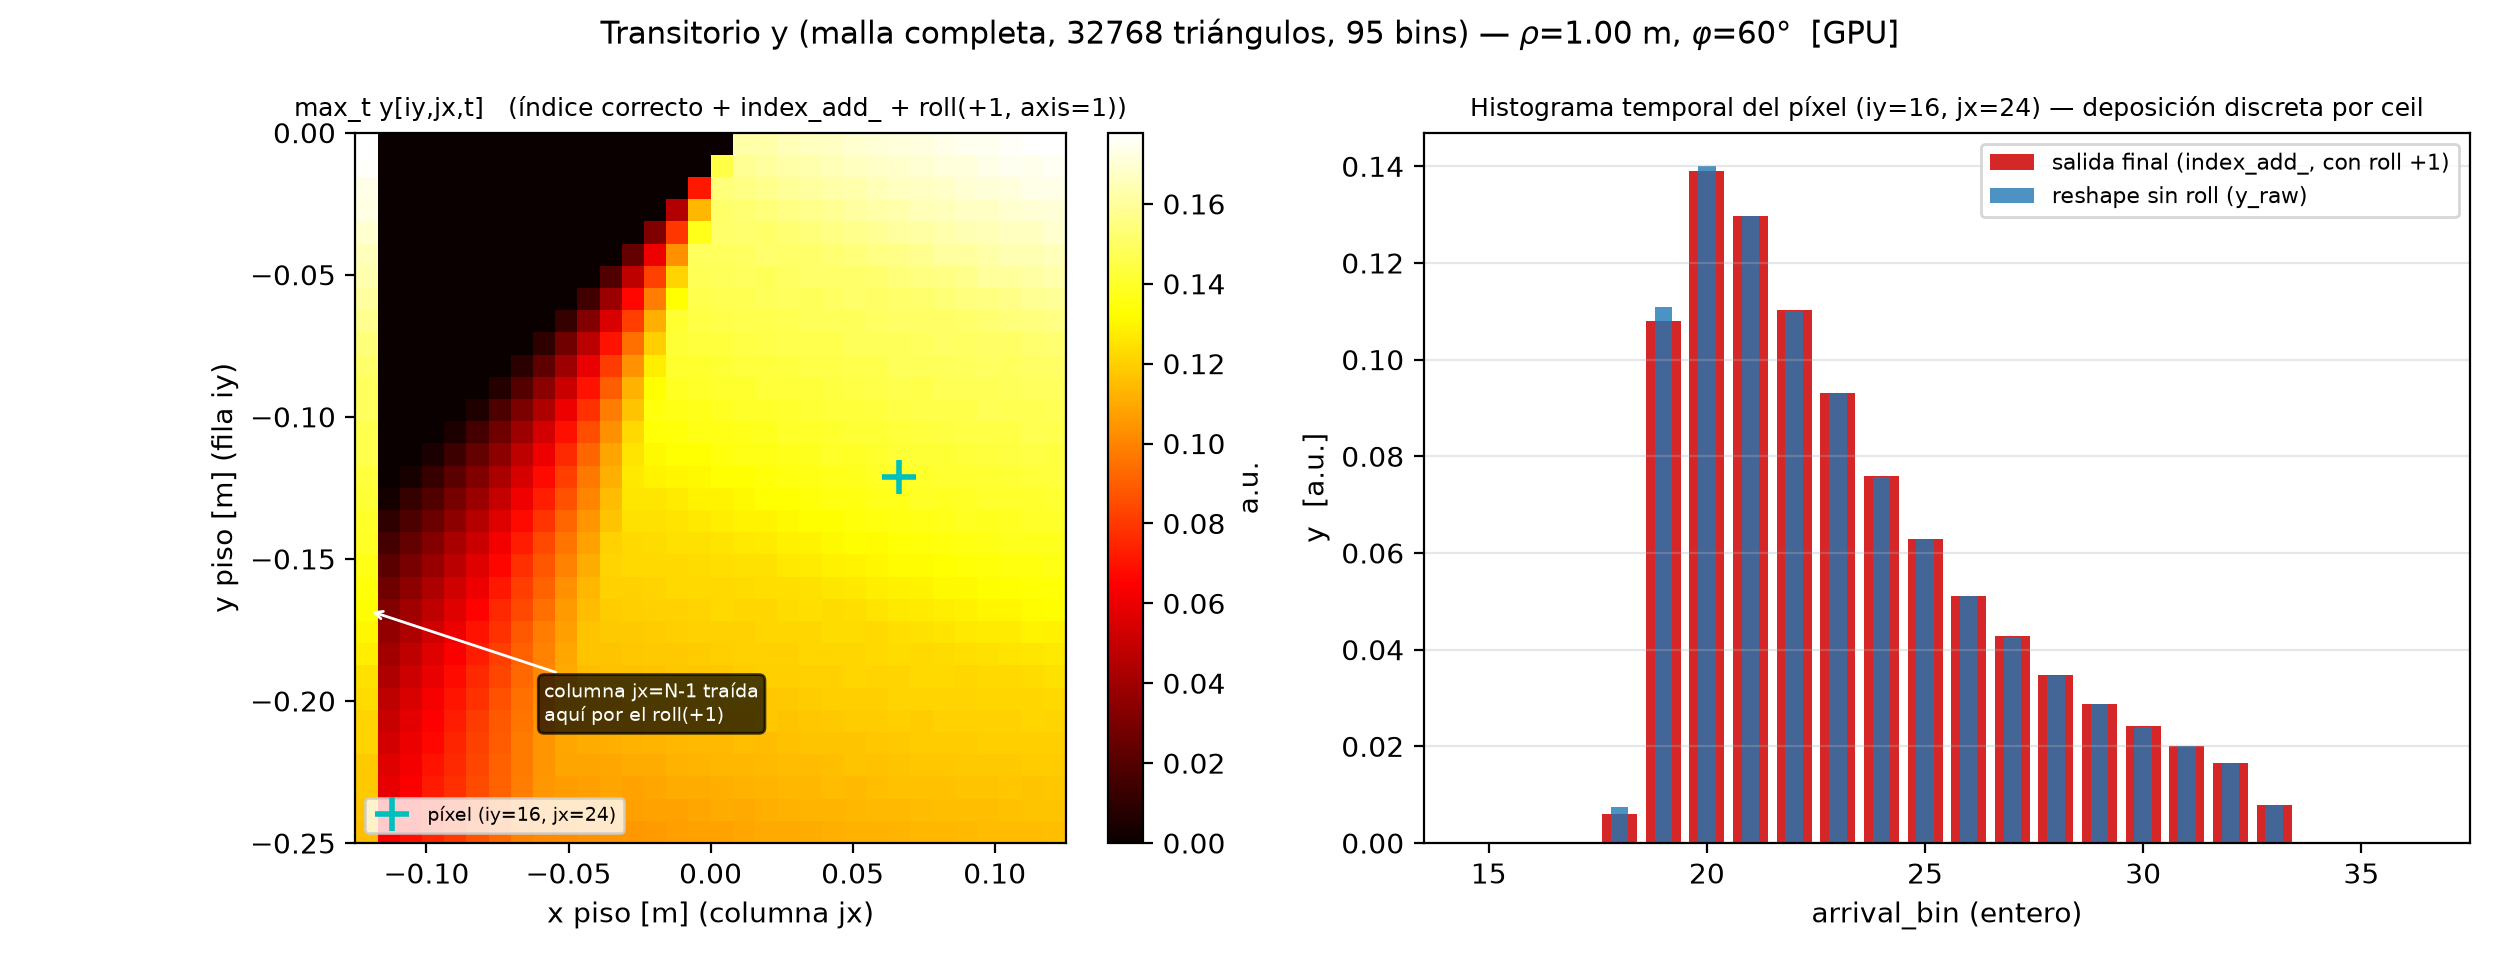
\includegraphics[width=\textwidth]{crb_sim_components_gpu_transient.png}}{%
  \fbox{\parbox{0.9\textwidth}{\centering\vspace{2em}(figura no
  disponible)\vspace{2em}}}}
\caption{El transitorio esperado con la malla completa de $32\,768$ triángulos.
Izquierda: máximo temporal por píxel; la cuña negra es la sombra del oclusor
(comparar con la máscara de la figura~\ref{fig:oclusion}) y la anotación señala
la columna que el \code{roll} trae desde el otro extremo. Derecha: histograma
temporal de un píxel, con y sin \code{roll} superpuestos; ocupa unos $16$
\emph{bins}.}
\label{fig:transitorio}
\end{figure}

\begin{obs}[Coste y validación de la vectorización]
El bucle sobre \code{triangle\_chunk\_size}$=256$ triángulos procesa un bloque
contra los $1024$ píxeles de golpe, en lugar de un triángulo por vez. Es
puramente una reorganización aritmética: una réplica independiente en
\code{numpy} del bucle fiel reproduce la salida de
\code{simulator.simulation} con error máximo $5.6\cdot10^{-17}$ (relativo
$3.1\cdot10^{-16}$), es decir, a precisión de máquina. El coste en CPU con
\code{float64} es de unos $1.2$--$1.7\,$s por evaluación a $32\times32$.
\end{obs}

%=======================================================================
\section{Del transitorio al modelo estadístico}
\label{sec:estadistico}

\subsection{Por qué Poisson}

El transitorio \eqref{eq:forward} es una \emph{tasa esperada}, no una medición.
Un SPAD no mide intensidad: cuenta fotones individuales. La estadística de ese
conteo es de Poisson por una razón fundamental: los fotones llegan como eventos
independientes en el tiempo, con una tasa instantánea proporcional a la
irradiancia, y el número de eventos de un proceso de Poisson en una ventana fija
sigue una distribución de Poisson. Que el detector sea de conteo de fotón único
hace que esta descripción sea exacta, no una aproximación de conveniencia: no
hay un ruido gaussiano aditivo dominante que la enmascare.

La consecuencia crucial para el CRB es que en Poisson
%
\begin{equation}
\label{eq:poisson-var}
\operatorname{Var}(x_q) = \E[x_q] = g_q ,
\end{equation}
%
la varianza \emph{es} la media. No hay un parámetro de ruido libre: el nivel de
señal fija por sí solo la incertidumbre. Esto es lo que hace que las constantes
radiométricas importen (salvedad~\ref{sal:constante}) y lo que da al peso
$1/g_q$ de la sección~\ref{sec:fisher} su interpretación.

\subsection{El fondo \texorpdfstring{$b$}{b}}

El modelo de medición es
%
\begin{equation}
\label{eq:g}
g_q(\vect\psi) = y_q(\vect\psi) + b,
\qquad b = 0.1\ \text{cuentas/\emph{bin}},
\end{equation}
%
para cada uno de los $q=1,\dots,97\,280$ índices (píxel, \emph{bin}). En el
código esto es \code{forward\_g\_polar} de \code{crb\_polar\_functions.py}, que
construye
%
\begin{center}
\code{background = background\_rate * ones\_like(y\_signal)}
\end{center}
%
y devuelve \code{y\_signal + background}. El valor $0.1$ es la constante
\code{BASELINE\_BACKGROUND\_RATE} de \code{crb\_fd\_baseline.py}.

Tiene dos justificaciones que se refuerzan:

\begin{itemize}[leftmargin=*]
  \item \textbf{Física}: un SPAD real tiene cuentas oscuras y recibe luz
        ambiente, así que ningún \emph{bin} tiene tasa exactamente cero. Un
        fondo plano es el modelo más simple de ese piso.
  \item \textbf{Matemática}: sin $b$, los \emph{bins} sin señal tendrían
        $g_q=0$ y el peso $1/g_q$ de \eqref{eq:fisher} divergería. Como la
        inmensa mayoría de los $97\,280$ índices no reciben señal ---solo unos
        $15$--$21$ \emph{bins} de cada píxel iluminado--- esto no es un detalle
        marginal sino la diferencia entre un problema bien planteado y una
        división por cero. Con $b=0.1$, el piso \code{fisher\_eps}$=10^{-12}$
        de \code{fisher\_poisson} nunca llega a actuar.
\end{itemize}

Conviene ser preciso sobre qué aporta $b$ al CRB: los índices con
$\partial g_q/\partial\vect\psi=0$ (los que nunca ven la faceta, para ninguna de
las perturbaciones) contribuyen \emph{cero} a la información, por muy grande que
sea $1/g_q$. El fondo no añade información; lo que hace es \textbf{diluir} la de
los \emph{bins} que sí tienen señal, porque aumenta su varianza sin aumentar su
sensibilidad. Subir $b$ empeora el CRB, como debe ser.

\subsection{El CRB no consume datos}

Una confusión frecuente merece una advertencia explícita. El CRB
\textbf{no usa mediciones ruidosas}. Se evalúa enteramente sobre el modelo
esperado: el \emph{pipeline} llama al simulador con \code{add\_noise=False}
(forzado, véase la sección~\ref{sec:adaptador}), de modo que $\vect y$ es la
tasa limpia y el \enquote{ruido} entra solo analíticamente, a través de la forma
de la verosimilitud de Poisson. No se generan realizaciones, no se promedia
sobre repeticiones y no hay semilla aleatoria. Por eso el cálculo es
determinista y reproducible bit a bit.

\subsection{Independencia entre índices}

La verosimilitud de la sección siguiente supone que los $97\,280$ conteos son
mutuamente independientes dado $\vect\psi$. Para el conteo de fotones esto es
razonable: distintos \emph{bins} temporales son ventanas disjuntas de un proceso
de Poisson, y distintos píxeles son detectores físicamente separados, de modo
que los eventos no se comparten.

\begin{salvedad}[Los límites de la independencia]
La suposición ignora tres efectos reales. El \emph{tiempo muerto} del SPAD:
tras una detección el píxel queda ciego un tiempo, lo que correlaciona
negativamente \emph{bins} consecutivos y, en régimen de flujo alto, sesga el
histograma hacia los \emph{bins} tempranos (\emph{pile-up}). La \emph{diafonía}
óptica y eléctrica entre píxeles vecinos. Y la \emph{jitter} temporal del
detector, que difumina la asignación de \emph{bin} y correlaciona vecinos. Nada
de esto está en el modelo, así que el CRB que sigue es el de un detector ideal:
optimista frente a un sensor real.
\end{salvedad}

%=======================================================================
\section{La información de Fisher}
\label{sec:fisher}

\subsection{Derivación}

Con conteos de Poisson independientes, la verosimilitud de una realización
$\vect x$ es $\prod_q e^{-g_q}g_q^{x_q}/x_q!$ y la log-verosimilitud
%
\begin{equation}
\label{eq:loglik}
\ell(\vect\psi) = \sum_q \bigl[\, x_q\ln g_q(\vect\psi) - g_q(\vect\psi)
- \ln x_q!\,\bigr].
\end{equation}
%
El último término no depende de $\vect\psi$ y desaparece al derivar. Derivando
respecto de la componente $m$-ésima del parámetro,
%
\begin{equation}
\label{eq:score}
\frac{\partial\ell}{\partial\psi_m}
= \sum_q \Bigl(\frac{x_q}{g_q}-1\Bigr)\frac{\partial g_q}{\partial\psi_m}
= \sum_q \frac{x_q-g_q}{g_q}\,\frac{\partial g_q}{\partial\psi_m} .
\end{equation}
%
Esta expresión es la \emph{score}. Nótese de paso que
$\E[\partial\ell/\partial\psi_m]=0$ porque $\E[x_q]=g_q$: el estimador de máxima
verosimilitud está bien centrado, como debe ser.

La información de Fisher es la covarianza de la \emph{score}:
%
\begin{equation}
\label{eq:def-fisher}
I_{mk} = \E\Bigl[\frac{\partial\ell}{\partial\psi_m}
                 \frac{\partial\ell}{\partial\psi_k}\Bigr]
       = \sum_{q}\sum_{q'}
         \frac{\E[(x_q-g_q)(x_{q'}-g_{q'})]}{g_q\,g_{q'}}
         \frac{\partial g_q}{\partial\psi_m}
         \frac{\partial g_{q'}}{\partial\psi_k} .
\end{equation}
%
Aquí es donde entra la independencia. Para $q\ne q'$ los conteos son
independientes y ambos factores tienen media cero, luego
$\E[(x_q-g_q)(x_{q'}-g_{q'})]=0$: \textbf{todos los términos cruzados se
anulan}. Para $q=q'$ queda la varianza, que por \eqref{eq:poisson-var} vale
$g_q$. Sustituyendo:
%
\begin{equation}
\label{eq:fisher}
\boxed{\ 
I_{mk}(\vect\psi) = \sum_q \frac{1}{g_q(\vect\psi)}
  \frac{\partial g_q}{\partial\psi_m}
  \frac{\partial g_q}{\partial\psi_k}\ }
\end{equation}
%
o, en forma matricial, con $\matr J_{qm}=\partial g_q/\partial\psi_m$ el
jacobiano de tamaño $97\,280\times2$,
%
\begin{equation}
\label{eq:fisher-mat}
\matr I = \matr J^\top \operatorname{diag}\!\bigl(1/\vect g\bigr)\, \matr J ,
\end{equation}
%
que es literalmente \code{crb\_polar\_functions.fisher\_poisson}:
%
\begin{center}
\code{g\_safe = np.maximum(g, eps)};\quad
\code{return J.T @ ((1.0/g\_safe)[:, None] * J)} .
\end{center}

\subsection{Cómo leerla}

Cada índice de medición contribuye a $\matr I$ un término
%
\[
\frac{(\partial g_q/\partial\psi_m)^2}{g_q}
= \frac{(\text{sensibilidad})^2}{\text{varianza}} ,
\]
%
que es la forma canónica de una relación señal--ruido. Un \emph{bin} informa
sobre $\rho$ en la medida en que (i) su tasa esperada \emph{cambia} al mover
$\rho$ y (ii) esa tasa no está ella misma dominada por fluctuación. Los dos
extremos aclaran la intuición: un \emph{bin} en el que la señal es enorme pero
insensible a la pose no aporta nada; un \emph{bin} muy sensible pero con tasa
casi nula tampoco, porque su propio ruido de Poisson lo ahoga --- salvo que
$g_q$ pequeño en el denominador lo amplifique, que es la razón por la que los
\emph{bins} del \emph{borde} del pulso, donde $g$ es bajo y la derivada alta,
son los más informativos.

Dos propiedades estructurales que se usarán después:
%
\begin{itemize}[leftmargin=*]
  \item $\matr I$ es una \textbf{suma sobre índices de medición}. De ahí la
        aditividad que explica el escalado con la resolución
        (sección~\ref{sec:baseline}).
  \item $\matr I$ es simétrica y semidefinida positiva por construcción
        (es de la forma $\matr B^\top\matr B$ con
        $\matr B=\operatorname{diag}(1/\sqrt{\vect g})\matr J$), lo que garantiza
        que sus autovalores son $\ge0$ y que la elipse de la
        sección~\ref{sec:elipse} está bien definida.
\end{itemize}

%=======================================================================
\section{El jacobiano por diferencias finitas}
\label{sec:fd}

Todo lo anterior necesita $\matr J=\partial\vect g/\partial\vect\psi$. El
\emph{forward} \eqref{eq:forward} contiene indicadores y un
$\lceil\cdot\rceil$, así que no hay derivada en forma cerrada. El
\emph{pipeline} la aproxima numéricamente.

\subsection{Diferencias centrales}

Para cada componente $m$ del parámetro,
%
\begin{equation}
\label{eq:fd}
\matr J_{:,m} \approx
\frac{\vect g(\vect\psi+\delta_m\vect e_m)-\vect g(\vect\psi-\delta_m\vect e_m)}
     {2\,\delta_m},
\qquad
\vect\delta = (\delta_\rho,\delta_\varphi) = (0.01\,\text{m},\ 0.5^\circ),
\end{equation}
%
implementado en \code{crb\_polar\_functions.finite\_difference\_jacobian\_polar}
y configurado por \code{BASELINE\_FD\_STEPS} en \code{crb\_fd\_baseline.py}.
Cada pose cuesta $1+2\cdot2=5$ evaluaciones del \emph{forward}: una central para
$\vect g$ y cuatro perturbadas para las dos columnas de $\matr J$.

\paragraph{Por qué centrales y no unilaterales.}
Desarrollando en serie una función suave,
%
\[
\frac{g(\psi+\delta)-g(\psi-\delta)}{2\delta}
= g'(\psi) + \frac{\delta^2}{6}g'''(\psi) + O(\delta^4),
\]
%
los términos de orden par se cancelan por simetría y el error es
$O(\delta^2)$, frente al $O(\delta)$ de $(g(\psi+\delta)-g(\psi))/\delta$. Para
el mismo $\delta$ la diferencia central es un orden más precisa, a costa de una
evaluación extra por columna. Es la elección correcta aquí, donde el
\emph{forward} es caro pero no prohibitivo.

\subsection{El problema honesto: el \emph{forward} es escalonado}

El desarrollo de Taylor anterior supone que $g$ es suave, y \textbf{no lo es}.
Tres operaciones lo rompen: el $\lceil\cdot\rceil$ del \emph{binning}
\eqref{eq:bin}, el indicador de oclusión $\mathbf 1[x_{\text{int}}>0]$
\eqref{eq:xint} y los $\max(0,\cdot)$ de los cosenos \eqref{eq:dots}. Las dos
primeras son constantes a trozos: su derivada es cero casi en todas partes y no
existe en un conjunto de saltos.

La escala del problema se cuantifica así. Un \emph{bin} vale
$c\Delta t = 11.69\,$cm de camino \eqref{eq:cdt}. Cuánto hay que mover $\rho$
para avanzar un \emph{bin} depende de la sensibilidad del camino,
$|\partial(d_1+d_2)/\partial\rho|$, que medida en la pose
$(1\,\text{m},90^\circ)$ vale $1.60$ (y no $2$: el tramo $d_1$ crece casi a
razón de uno, pero $d_2$ crece más despacio porque el parche observado no está
en el origen sino desplazado a $(0,-0.125)$). Por tanto
%
\begin{equation}
\label{eq:paso-bin}
\Delta\rho_{\text{bin}}
= \frac{c\,\Delta t}{|\partial(d_1+d_2)/\partial\rho|}
= \frac{0.1169\,\text{m}}{1.60} = 7.3\,\text{cm} ,
\end{equation}
%
mientras que la diferencia central abarca $2\delta_\rho = 2\,$cm, es decir
\textbf{el 27\% de un \emph{bin}}. La consecuencia es directa: para
un \emph{triángulo aislado}, las dos evaluaciones $\vect g(\rho\pm\delta_\rho)$
caen casi siempre en el \emph{mismo} \emph{bin}, la diferencia es cero y la
derivada estimada es $0$; y cuando por casualidad cruzan un borde, salta una
masa entera y la derivada estimada es $\propto1/(2\delta_\rho)$. Ni una ni otra
es la derivada de nada.

\subsection{Por qué funciona a pesar de todo}

Dos mecanismos de promediado rescatan el cálculo, y ambos son consecuencia de
decisiones de modelado que ya justificamos por otras razones.

\begin{enumerate}[leftmargin=*]
  \item \textbf{La densificación a $32\,768$ triángulos.} Cada triángulo tiene
        su propio camino $d_1+d_2$ y por tanto su propio umbral de salto. Los
        umbrales están repartidos casi uniformemente en el intervalo de un
        \emph{bin}, porque la faceta mide $1.585\,$m de alto y los caminos se
        distribuyen de forma continua. Al mover $\rho$ en $\delta_\rho$, una
        \emph{fracción} bien definida de los triángulos cruza su umbral, y esa
        fracción es aproximadamente proporcional a $\delta_\rho$. La suma
        \eqref{eq:cuadratura} convierte así una colección de escalones en una
        rampa: el agregado es aproximadamente lineal aunque cada sumando sea una
        escalera. Esto es exactamente lo que se ve en el panel central de la
        figura~\ref{fig:cuantizacion}.
  \item \textbf{La suma sobre índices de medición en \eqref{eq:fisher}.} La
        información no depende de la derivada de un píxel, sino de la suma de
        $97\,280$ contribuciones. Los residuos de discretización que quedan
        tienen signos distintos según el píxel y se cancelan parcialmente.
\end{enumerate}

El panel derecho de la figura~\ref{fig:cuantizacion} pone a prueba esta
explicación de la única manera honesta: variando $\delta_\rho$ y viendo si el
resultado se mueve. Si el jacobiano fuese ruido de discretización, las
$\sigma$ salta\-rían de forma errática con el paso. Lo medido en
$(1\,\text{m},90^\circ)$ es esto:
%
\begin{center}
\small
\begin{tabular}{@{}lrrrrrr@{}}
\toprule
$\delta_\rho$ [mm] & 2 & 5 & 10 & 20 & 40 & 80 \\
\midrule
$\sigma_\rho$ [mm] & 8.512 & 8.724 & 8.795 & 9.015 & 9.708 & 10.808 \\
$\sigma_\varphi$ [$^\circ$] & 2.5742 & 2.5741 & 2.5741 & 2.5752 & 2.5754 & 2.5576 \\
\bottomrule
\end{tabular}
\end{center}
%
La lectura es tranquilizadora en dos sentidos. $\sigma_\varphi$ es
\emph{plana}, con variación total del 0.7\% sobre un rango de pasos de $40:1$,
como debe ser: $\delta_\rho$ solo afecta a la columna de $\rho$ del jacobiano.
Y $\sigma_\rho$ crece \textbf{monótona y suavemente} con el paso ---un
$27\%$ al pasar de $2$ a $80\,$mm---, que es la firma de un error de
truncamiento $O(\delta^2)$ sobre una respuesta efectivamente suave, no la de un
ruido de cuantización, que produciría saltos sin orden. El valor de referencia
$\delta_\rho=10\,$mm queda a un $3\%$ del extrapolado a paso cero. Nada de
esto \emph{demuestra} que el modelo sea diferenciable; muestra que el
promediado descrito arriba funciona lo bastante bien como para que el resultado
no dependa de forma crítica de una elección arbitraria.

\begin{figure}[htbp]
\centering
\IfFileExists{figs_forward/cuantizacion_rho.png}{%
  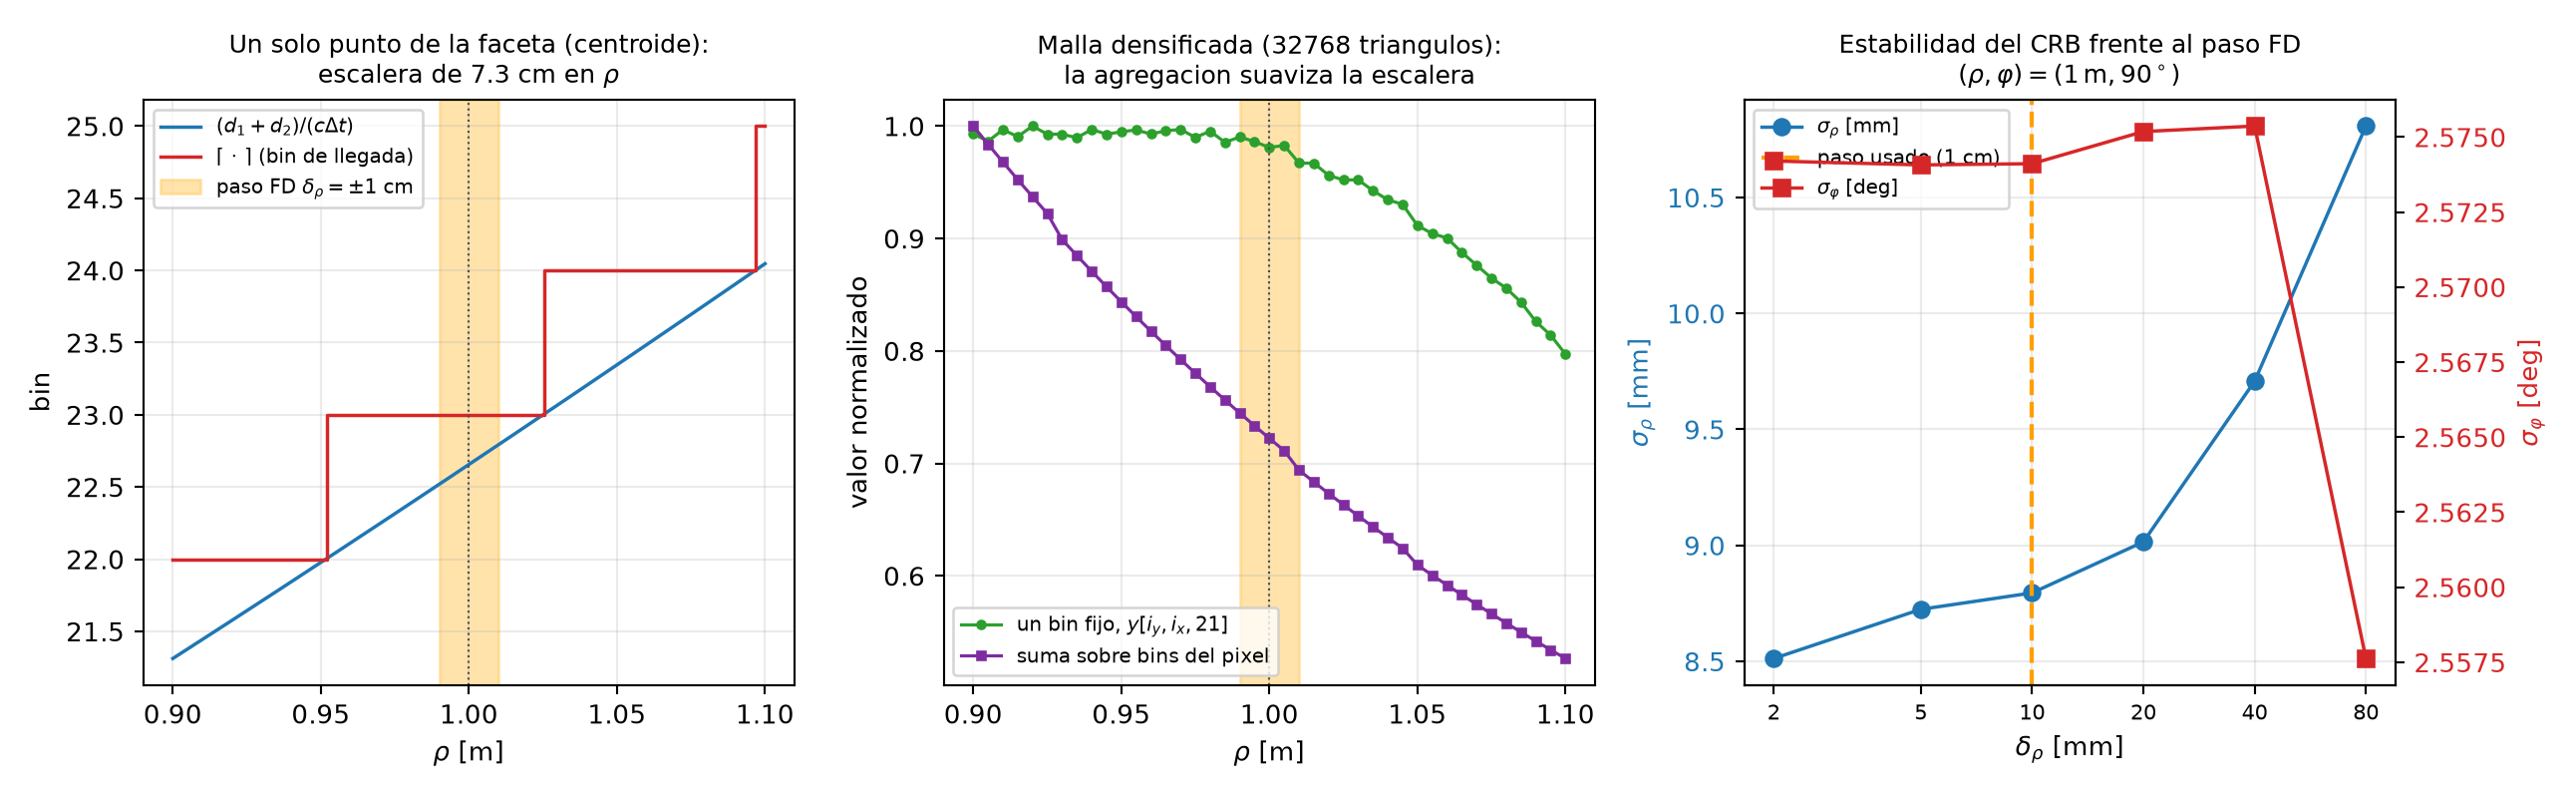
\includegraphics[width=\textwidth]{cuantizacion_rho.png}}{%
  \fbox{\parbox{0.9\textwidth}{\centering\vspace{2em}(figura
  \code{cuantizacion\_rho.png} no disponible)\vspace{2em}}}}
\caption{Por qué un paso de $1\,$cm funciona sobre un \emph{forward} cuantizado
en $7.3\,$cm de rango. Izquierda: para un punto fijo de la faceta el
\emph{bin} de llegada es una escalera, y la ventana del paso FD (banda
amarilla) cabe holgadamente dentro de una meseta, de modo que la derivada de
\emph{ese} punto sería exactamente cero. Centro: con la malla densificada, tanto
un \emph{bin} fijo como la suma del píxel responden de forma suave a $\rho$;
esta es la razón por la que la diferencia finita tiene sentido. Derecha:
$\sigma_\rho$ y $\sigma_\varphi$ frente al paso $\delta_\rho$, en escala
logarítmica; nótese la escala del eje de $\sigma_\varphi$, que abarca menos
del 1\%. Generada por \code{docs/figs\_forward/make\_aux\_figs.py}.}
\label{fig:cuantizacion}
\end{figure}

Una ilustración complementaria del mismo fenómeno está en la
figura~\ref{fig:suave}: si se sustituyera el $\lceil\cdot\rceil$ duro por un
núcleo suave, la escalera de la faceta real se convertiría en la curva continua
que el agregado ya aproxima de hecho. Es la idea que desarrolla la ruta
analítica documentada en \code{reporte\_consolidado.pdf}, y que reproduce a esta
ruta FD dentro de un 10\%.

\begin{figure}[htbp]
\centering
\IfFileExists{../gpu_vs_cpu/binning_smooth_overlay.png}{%
  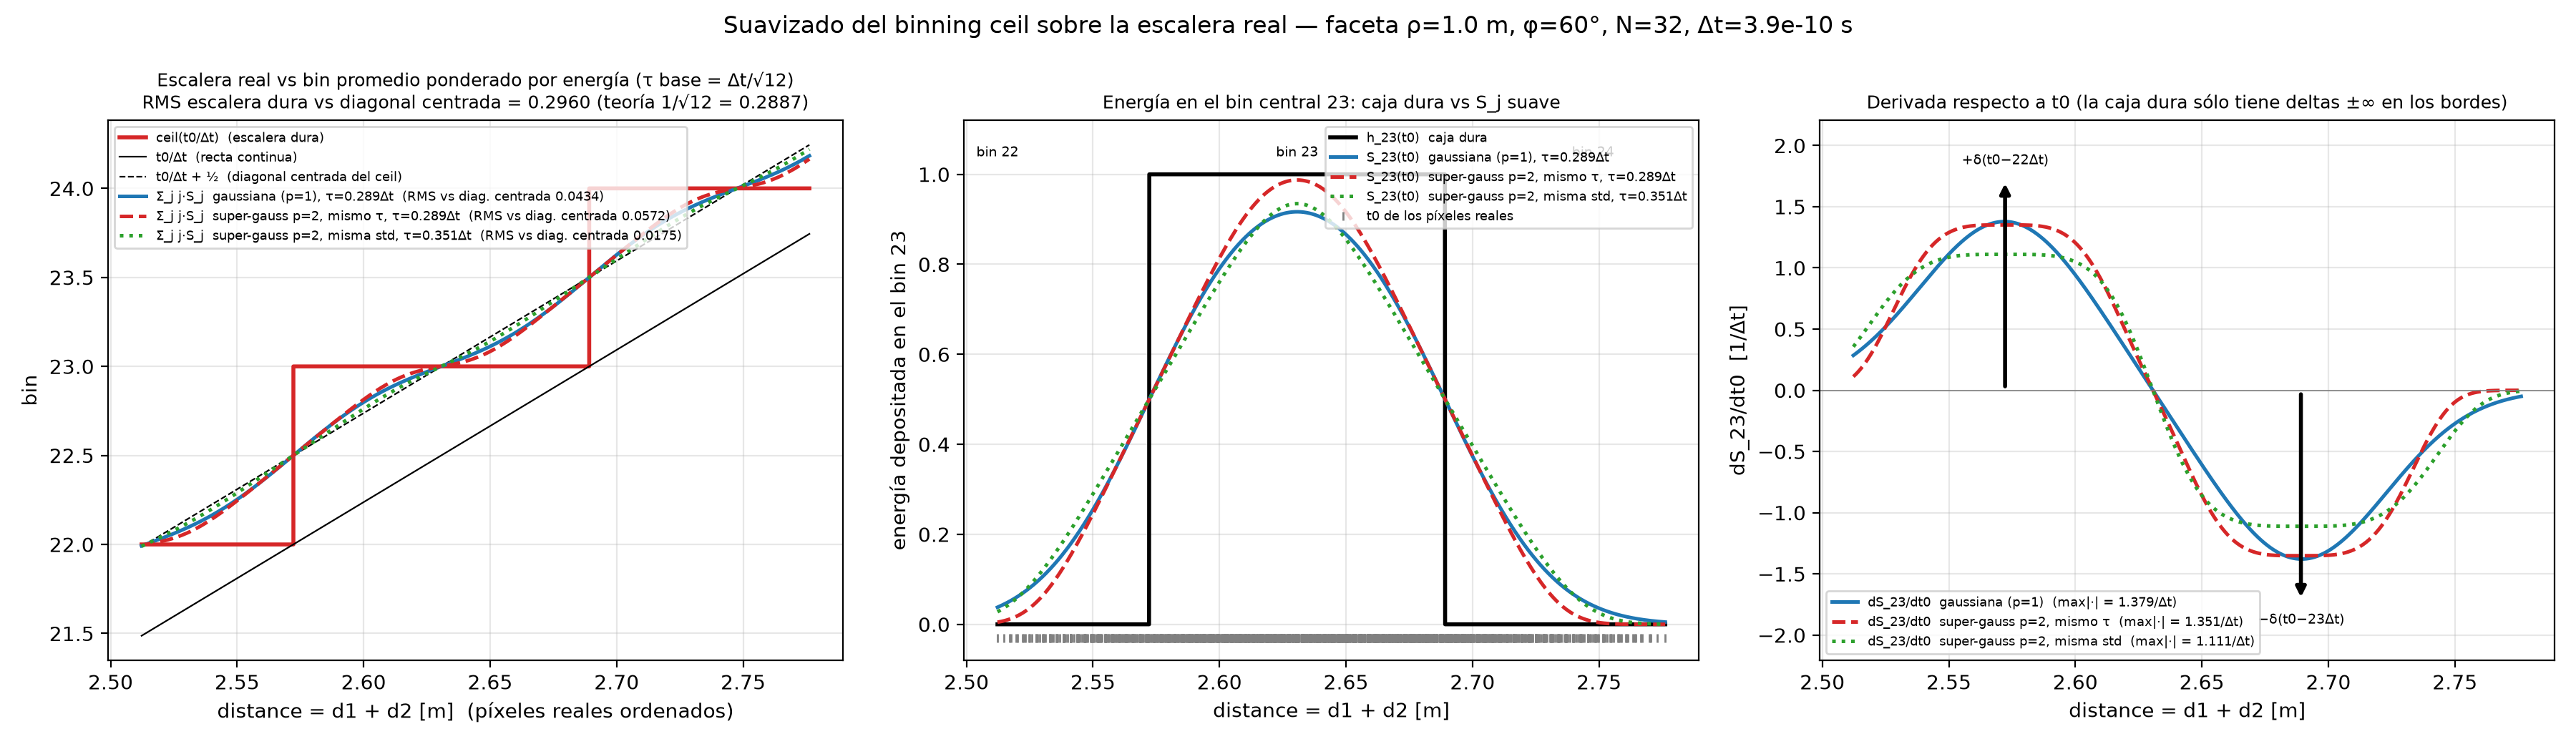
\includegraphics[width=0.92\textwidth]{binning_smooth_overlay.png}}{%
  \fbox{\parbox{0.9\textwidth}{\centering\vspace{2em}(figura no
  disponible)\vspace{2em}}}}
\caption{Suavizado del \emph{binning} sobre la escalera de la faceta real,
generado por \code{plot\_binning\_smoothing.py}: la cuantización dura frente a
su versión con núcleo, que es la que tiene derivada clásica.}
\label{fig:suave}
\end{figure}

\subsection{Por qué \code{float64}}

El \emph{baseline} fija \code{torch\_dtype = torch.float64} en
%
\begin{center}
\code{crb\_fd\_baseline.baseline\_simulation\_kwargs} .
\end{center}
%
La razón es el numerador
de \eqref{eq:fd}: se resta un par de números casi iguales y se divide
por un número pequeño. Con $\delta_\rho=1\,$cm la diferencia relativa entre
$\vect g(\rho+\delta)$ y $\vect g(\rho-\delta)$ es del orden de $10^{-2}$, y el
épsilon relativo de \code{float32} es $\approx1.2\cdot10^{-7}$: la cancelación
catastrófica dejaría unos cinco dígitos significativos, que se propagarían
elevados al cuadrado a $\matr I$. Con \code{float64} ($\epsilon\approx
2.2\cdot10^{-16}$) el margen es amplísimo. El coste es un factor $\sim2$ en
tiempo, irrelevante frente al riesgo.

\subsection{El adaptador de dos a tres valores}
\label{sec:adaptador}

Hay una incompatibilidad de interfaz que conviene documentar aquí, porque es lo
que conecta las secciones~\ref{sec:sim} y~\ref{sec:fisher} en el código.
La función
%
\begin{center}
\code{crb\_polar\_functions.simulate\_facet\_signal\_expected}
\end{center}
%
desempaqueta \textbf{tres} valores del \emph{callable} de simulación,
%
\begin{center}
\code{\_, y\_signal, params = simulation\_fn(**kwargs)} ,
\end{center}
%
herencia del simulador antiguo del \emph{notebook}, que devolvía la terna
\code{(ruidoso, limpio, params)}. El simulador nuevo devuelve
\textbf{dos} valores, \code{(y\_meas\_vec\_noisy, params)}.

Se adaptó el lado del CRB, no el simulador. El adaptador
%
\begin{center}
\code{crb\_fd\_baseline.simulation\_fn\_for\_crb}
\end{center}
%
llama a \code{simulator.simulation} y re-emite su par como la terna
$(\vect y,\vect y,\text{params})$. La operación es legítima porque el CRB
siempre invoca el \emph{forward} con \code{force\_no\_noise=True}, que fija
\code{add\_noise=False}; en ese caso el único transitorio devuelto \emph{es} la
tasa esperada sin ruido y puede ocupar ambas ranuras sin ambigüedad. El
adaptador falla de forma explícita si se le pasa \code{add\_noise=True}, para
que nunca se pueda calcular una \enquote{Fisher} sobre una realización
ruidosa. Con este diseño, \code{crb\_polar\_functions.py} no se modificó.

%=======================================================================
\section{La cota de Cramér--Rao}
\label{sec:crb}

\subsection{El enunciado y su alcance}

La desigualdad de Cramér--Rao dice que, para cualquier estimador
$\hat{\vect\psi}(\vect x)$ \textbf{insesgado} de $\vect\psi$,
%
\begin{equation}
\label{eq:crb}
\Cov(\hat{\vect\psi}) \;\succeq\; \matr I(\vect\psi)^{-1} ,
\end{equation}
%
donde $\succeq$ significa que la diferencia es semidefinida positiva. Tomando
elementos diagonales, $\operatorname{Var}(\hat\rho)\ge[\matr I^{-1}]_{11}$ y
análogamente para $\varphi$. El \emph{pipeline} define
%
\begin{equation}
\label{eq:sigmas}
\matr C = \matr I^{-1},\qquad
\sigma_\rho=\sqrt{C_{11}},\qquad
\sigma_\varphi=\sqrt{C_{22}},\qquad
\sigma_{\text{tang}} = \rho\,\sigma_\varphi ,
\end{equation}
%
en \code{compute\_crb\_polar} y \code{\_crb\_sigmas\_from\_matrix}. El error
tangencial $\rho\,\sigma_\varphi$ convierte la incertidumbre angular a metros
sobre el arco, para poderla comparar con $\sigma_\rho$ en las mismas unidades.

\paragraph{La inversión es una pseudoinversa.}
El código usa \code{CRB = np.linalg.pinv(I)} y no \code{inv}. La razón es
robustez: si en alguna pose una dirección del espacio de parámetros no fuera
observable, $\matr I$ sería singular y \code{inv} lanzaría una excepción,
abortando la rejilla entera. La pseudoinversa devuelve el mejor sustituto
(anulando la dirección no informativa) y permite detectar el problema mirando
las $\sigma$. En la rejilla \emph{baseline} $\matr I$ está bien condicionada en
las $15$ poses y \code{pinv} coincide con \code{inv}.

\paragraph{Qué no dice la cota.}
Tres precisiones que evitan sobreinterpretarla:
%
\begin{itemize}[leftmargin=*]
  \item Es una \textbf{cota inferior}, no el error de un estimador concreto.
        Ningún estimador tiene que alcanzarla; el de máxima verosimilitud la
        alcanza asintóticamente en muchos casos regulares, pero aquí el
        \emph{forward} es escalonado y esa garantía no aplica sin más.
  \item Vale para estimadores \textbf{insesgados}. Un estimador sesgado puede
        tener varianza menor (el caso extremo, $\hat{\vect\psi}=$ constante,
        tiene varianza cero), a costa del sesgo.
  \item Es \textbf{local}: $\matr I$ se evalúa en un $\vect\psi$ concreto y
        describe la curvatura de la verosimilitud ahí. No dice nada sobre
        ambigüedades globales, por ejemplo dos poses muy separadas que produzcan
        transitorios parecidos.
\end{itemize}

\subsection{La correlación entre \texorpdfstring{$\rho$ y $\varphi$}{rho y phi}}
\label{sec:corr}

El elemento fuera de la diagonal es tan informativo como los de la diagonal, y
se reporta como
%
\begin{equation}
\label{eq:corr}
r_{\rho\varphi} = \frac{C_{12}}{\sqrt{C_{11}C_{22}}}
\qquad\text{(columna \code{corr} de la tabla \emph{baseline})}.
\end{equation}

\paragraph{Por qué $I_{\rho\varphi}\ne0$.}
Mirando \eqref{eq:fisher}, $I_{\rho\varphi}=\sum_q
g_q^{-1}(\partial_\rho g_q)(\partial_\varphi g_q)$ se anula solo si ninguna
medición es sensible a ambos parámetros a la vez. Aquí ocurre lo contrario, por
dos vías:
%
\begin{itemize}[leftmargin=*]
  \item el \textbf{camino} $d_1+d_2$ depende de la posición
        $(\rho\cos\varphi,\rho\sin\varphi)$, es decir de \emph{ambas}
        coordenadas: girar la faceta también cambia su distancia al parche
        observado, que no está centrado en el origen sino en $(0,-0.125)$;
  \item la \textbf{oclusión} $x_{\text{int}}$ \eqref{eq:xint} depende de la
        posición completa del centroide, así que mover $\rho$ desplaza también
        la frontera de la sombra, que es el mecanismo por el que se mide
        $\varphi$.
\end{itemize}

\paragraph{Qué significa el signo.}
Todas las correlaciones de la rejilla \emph{baseline} son \textbf{negativas}. Un
$r_{\rho\varphi}<0$ dice que los errores están anticorrelacionados: una
sobreestimación de $\rho$ tiende a acompañarse de una subestimación de
$\varphi$. La lectura física es que existe una \textbf{dirección de
compensación} en el plano $(\rho,\varphi)$ a lo largo de la cual el transitorio
cambia poco: alejar la faceta y girarla hacia el hueco produce, hasta primer
orden, un camino y una sombra parecidos. El estimador puede distinguir bien un
desplazamiento perpendicular a esa dirección y mal uno paralelo a ella; de ahí
que las elipses de la sección~\ref{sec:elipse} salgan alargadas e inclinadas.

\paragraph{Los valores medidos.}
La correlación no es uniforme sobre la rejilla: es más fuerte de cerca y con la
faceta hacia el borde iluminado, y más débil de lejos.
%
\begin{center}
\begin{tabular}{@{}lrrr@{}}
\toprule
$r_{\rho\varphi}$ & $\varphi=30^\circ$ & $\varphi=90^\circ$ & $\varphi=150^\circ$ \\
\midrule
$\rho=0.5\,$m & $-0.731$ & $-0.435$ & $-0.403$ \\
$\rho=1.0\,$m & $-0.564$ & $-0.283$ & $-0.256$ \\
$\rho=1.5\,$m & $-0.452$ & $-0.209$ & $-0.184$ \\
\bottomrule
\end{tabular}
\end{center}
%
El recorrido completo va de $-0.731$ en $(0.5\,\text{m},30^\circ)$ a $-0.184$ en
$(1.5\,\text{m},150^\circ)$; la tabla~\ref{tab:baseline} da las $15$ poses.

\begin{obs}[Independientes como coordenadas, dependientes como estimadores]
\label{obs:indep}
$\rho$ y $\varphi$ son coordenadas independientes: se pueden fijar por separado
y nada las liga \emph{a priori}. Lo que está correlacionado son los
\textbf{errores de sus estimaciones}, porque los datos no las separan
limpiamente. Son dos afirmaciones sobre objetos distintos: una sobre la
parametrización, otra sobre la geometría de la verosimilitud.
\end{obs}

\begin{obs}[Las $\sigma$ son conjuntas, no condicionales]
Los $\sigma_\rho$ y $\sigma_\varphi$ de \eqref{eq:sigmas} salen de invertir la
matriz $2\times2$ \emph{completa}: son las incertidumbres de estimar los dos
parámetros \emph{a la vez}. La incertidumbre \emph{condicional} (conociendo
$\varphi$ de antemano) sería $1/\sqrt{I_{\rho\rho}}$, y la relación entre ambas
es
%
\[
\sigma_\rho = \frac{1}{\sqrt{I_{\rho\rho}}}\cdot
              \frac{1}{\sqrt{1-r_I^2}},
\qquad
r_I=\frac{I_{\rho\varphi}}{\sqrt{I_{\rho\rho}I_{\varphi\varphi}}} ,
\]
%
de modo que la incertidumbre conjunta es siempre \textbf{mayor} o igual que la
condicional, y el factor de inflación crece al acercarse la correlación a $\pm1$.
Estimar un parámetro extra nunca sale gratis. Este es el mismo mecanismo por el
que, en la ruta antigua de tres parámetros, añadir la altura $h$ ensanchaba
todas las burbujas.
\end{obs}

%=======================================================================
\section{De la matriz a la elipse}
\label{sec:elipse}

\subsection{La región de confianza es una elipse}

Dada la matriz de covarianza $\matr C$ (aquí el CRB), el conjunto
%
\begin{equation}
\label{eq:region}
\mathcal E_k = \bigl\{\vect\delta\in\mathbb R^2:\
\vect\delta^\top \matr C^{-1}\vect\delta \le k^2 \bigr\}
\end{equation}
%
es un elipsoide (en dimensión $2$, una elipse) centrado en el origen. Su
frontera se parametriza de forma explícita mediante la descomposición espectral.
Como $\matr C$ es simétrica y definida positiva, existe
%
\begin{equation}
\label{eq:eig}
\matr C = \matr V\matr\Lambda\matr V^\top,
\qquad \matr\Lambda=\operatorname{diag}(\lambda_1,\lambda_2),\quad
\matr V \text{ ortogonal},
\end{equation}
%
y sustituyendo $\vect\delta=\matr V\matr\Lambda^{1/2}\vect u$ en
\eqref{eq:region} la condición se vuelve $\lVert\vect u\rVert\le k$. Por tanto la
frontera es la imagen de un círculo de radio $k$:
%
\begin{equation}
\label{eq:ellipse}
\vect\delta(\vartheta)
= k\,\matr V \matr\Lambda^{1/2}
  \begin{pmatrix}\cos\vartheta\\ \sin\vartheta\end{pmatrix},
\qquad \vartheta\in[0,2\pi) ,
\end{equation}
%
es decir: \textbf{semiejes $k\sqrt{\lambda_i}$, orientados según los
autovectores de $\matr C$}. Esto es exactamente
\code{crb\_region\_in\_polar\_parameters}:
%
\begin{center}
\code{eigenvalues, eigenvectors = np.linalg.eigh(Sigma)};\quad
\code{axes = k * np.sqrt(eigenvalues)};\\
\code{ellipse = center[:,None] + eigenvectors @ np.diag(axes) @ circle} ,
\end{center}
%
con \code{circle} el círculo unidad muestreado en \code{n\_points=300} y
\code{np.maximum(eigenvalues, 0.0)} como guarda contra autovalores
ligerísimamente negativos por redondeo.

\subsection{Por qué \texorpdfstring{$k=3$}{k=3}}

Si los errores fueran gaussianos de covarianza $\matr C$, la forma cuadrática
$\vect\delta^\top\matr C^{-1}\vect\delta$ seguiría una $\chi^2$ con $2$ grados
de libertad, cuya función de distribución es $F(u)=1-e^{-u/2}$. Con $k=3$,
%
\begin{equation}
\label{eq:cobertura}
\Pr\bigl(\vect\delta\in\mathcal E_3\bigr) = 1-e^{-k^2/2} = 1-e^{-4.5}
= 0.98889 ,
\end{equation}
%
es decir, la región $\mathcal E_3$ contiene el 98.9\% de la masa de
probabilidad.

\begin{obs}[La regla de $3\sigma$ en 2D no es la de 1D]
En una dimensión, $\pm3\sigma$ cubre el 99.73\%. En dos dimensiones la
misma $k$ cubre solo el 98.89\%, porque hay \enquote{más sitio} fuera: la
masa de probabilidad se reparte en un anillo cuyo perímetro crece con el radio.
Conviene citar el número correcto, 98.9\%, y no el de 1D.
\end{obs}

\subsection{La inclinación \emph{es} la correlación}

La orientación de la elipse y la correlación de la sección~\ref{sec:corr} son la
misma información vista de dos formas. Si $r_{\rho\varphi}=0$, la matriz
$\matr C$ es diagonal, sus autovectores son los ejes coordenados y la elipse
sale \textbf{alineada} con ellos. Si $r_{\rho\varphi}\ne0$, los autovectores
giran; el ángulo de giro satisface
%
\begin{equation}
\label{eq:tilt}
\tan(2\alpha) = \frac{2C_{12}}{C_{11}-C_{22}} ,
\end{equation}
%
y el signo de $C_{12}$ determina hacia qué lado. Con $C_{12}<0$ en toda la
rejilla, el eje mayor de las elipses apunta en la dirección de compensación
\enquote{$\rho$ arriba, $\varphi$ abajo}: mirar la inclinación de una burbuja es
leer directamente qué combinación de rango y ángulo el sensor no consigue
separar.

\subsection{Por qué se dibuja en el espacio de parámetros}

Hay dos formas de representar la región, y el \emph{pipeline} usa
deliberadamente la primera.

\paragraph{Burbujas: la región en el plano $(\rho,\varphi)$.}
Es \eqref{eq:ellipse} tal cual, centrada en $(\rho_0,\varphi_0)$. Se elige esta
porque \textbf{el CRB vive en el espacio de parámetros}: es una cota sobre la
covarianza de $\hat{\vect\psi}=(\hat\rho,\hat\varphi)$, y sus semiejes son
literalmente las incertidumbres que se quieren leer. No hay ninguna
transformación intermedia que pueda introducir error o confundir la
interpretación.

\paragraph{Gotas: el empuje al plano físico $xy$.}
La alternativa es transportar la región a la posición física mediante la
linealización de $(x,y)=(\rho\cos\varphi,\rho\sin\varphi)$:
%
\begin{equation}
\label{eq:pushforward}
\matr A = \frac{\partial(x,y)}{\partial(\rho,\varphi)}
= \begin{pmatrix}\cos\varphi & -\rho\sin\varphi\\
                 \sin\varphi & \rho\cos\varphi\end{pmatrix},
\qquad
\matr\Sigma_{xy} = \matr A\,\matr C\,\matr A^\top ,
\end{equation}
%
que es lo que implementa \code{crb\_region\_physical\_xy\_to\_polar} (existe en
el módulo y está disponible con
\code{plot\_crb\_regions\_polar(..., use\_physical\_region=True)}). Tiene dos
inconvenientes. Primero, \eqref{eq:pushforward} es una \textbf{aproximación de
primer orden}: la aplicación polar$\to$cartesiana no es lineal, así que la
imagen exacta de una elipse no es una elipse, y cuanto mayor sea
$\rho\,\sigma_\varphi$ frente a $\rho$ más se deforma. Segundo, al reconvertir a
polares para dibujar sobre el eje polar, el contorno se curva y adopta la forma
de gota que motivó abandonar esta representación: visualmente sugiere una
asimetría que no está en el CRB, sino en el cambio de coordenadas.

El \emph{pipeline} usa por tanto
%
\begin{center}
\code{plot\_crb\_regions\_polar(results, use\_physical\_region=False, rlim=2.0, ...)}
\end{center}
%
que selecciona las claves \code{rho\_curve\_param} y \code{phi\_curve\_param}, y
dibuja sobre un eje polar con \code{ax.plot(phi\_curve, rho\_curve)}: $\varphi$
como coordenada angular y $\rho$ como radial. El estilo lo fija
\code{\_style\_polar\_crb\_ax}: medio plano $\theta\in[0,180^\circ]$, cero a la
derecha (\code{set\_theta\_zero\_location("E")}), sentido antihorario,
etiquetas radiales a dos decimales y fuentes reducidas.

\begin{obs}[Por qué las burbujas se ven \enquote{arqueadas}]
Las elipses de la figura~\ref{fig:baseline} no son elipses perfectas en la
página, sino curvas arqueadas. No es una deformación del CRB: es que se está
dibujando una elipse del plano cartesiano $(\varphi,\rho)$ sobre unos
\emph{ejes polares}. Un segmento de $\rho$ constante es un arco de
circunferencia en el papel, así que la elipse aparece curvada. Es una
consecuencia puramente gráfica de haber elegido un eje polar para que la
posición de cada burbuja coincida con la dirección física de la pose.
\end{obs}

\begin{salvedad}[Unidades mixtas en el plano de la elipse]
\label{sal:unidades}
El plano $(\rho,\varphi)$ mezcla metros y radianes, de modo que
\enquote{semieje} y \enquote{ángulo de inclinación} dependen de la escala
relativa que se elija entre los dos ejes. Los autovalores de \eqref{eq:eig} no
son invariantes geométricos; cambiar $\varphi$ de radianes a grados cambiaría
los semiejes y la inclinación. No es un error, es una convención: mientras se
aplique la misma a todas las poses y a todos los métodos, las comparaciones son
válidas. Lo que sí es invariante son las cantidades escalares $\sigma_\rho$ y
$\sigma_\varphi$ por separado, y su combinación en unidades homogéneas
$\rho\,\sigma_\varphi$.
\end{salvedad}

%=======================================================================
\section{El \emph{baseline} de \texorpdfstring{$32\times32$}{32x32}}
\label{sec:baseline}

\subsection{Cómo escala la precisión con la resolución}

De la estructura de \eqref{eq:fisher} sale una predicción cuantitativa.
$\matr I$ es una suma sobre índices de medición, y los índices son
$(\text{píxel},\text{\emph{bin}})$. Al pasar de $N\times N$ a $2N\times2N$
píxeles con el mismo FOV, el número de píxeles se cuadruplica. La pregunta es
qué le pasa a la contribución de cada píxel.

Aquí hay un detalle del modelo que conviene explicitar: la
intensidad~\eqref{eq:intensity} \textbf{no lleva ningún factor de área de
píxel}. El simulador \emph{muestrea} la radiancia del suelo en el centro de cada
píxel; no la integra sobre su huella. Por tanto, al refinar la grilla, cada
píxel conserva aproximadamente su valor esperado y simplemente hay cuatro veces
más de ellos. Entonces
%
\begin{equation}
\label{eq:escalado}
\matr I \propto N_{\text{px}} = N^2
\quad\Longrightarrow\quad
\sigma \propto \frac{1}{\sqrt{N_{\text{px}}}} = \frac{1}{N} .
\end{equation}

\begin{salvedad}[Este escalado es del modelo, no de la física]
\label{sal:escalado}
Un sensor real con FOV fijo recoge un flujo de fotones fijo; subdividirlo en más
píxeles \emph{reparte} esos fotones, y la información total se mantendría
aproximadamente constante. La ley \eqref{eq:escalado} aparece porque el modelo
puntual multiplica el número de muestras sin dividir la señal entre ellas. Es
consistente y útil para comparar configuraciones, pero no debe leerse como
\enquote{poner más píxeles mejora la precisión física}: describe cómo cambia el
CRB de \emph{este} modelo. Para modelar el reparto habría que multiplicar
\eqref{eq:intensity} por la huella del píxel, $(\text{FOV}/N)^2$.
\end{salvedad}

El barrido de \code{sr\_crb.py} (que usa \code{utils/crb\_utils.py} sobre el
mismo \emph{forward} y el mismo estimador) confirma \eqref{eq:escalado} con
precisión notable. En la pose $(\rho,\varphi)=(1\,\text{m},90^\circ)$:

\begin{table}[htbp]
\centering
\caption{Barrido de resolución en $(1\,\text{m},90^\circ)$, de
\code{sr\_crb.py --pixel-dims 8,16,32,64}. La última columna compara con la
predicción $\sigma\propto1/N$ tomando $N=8$ como referencia.}
\label{tab:sweep}
\begin{tabular}{@{}rrrrr@{}}
\toprule
$N$ & $\sigma_\rho$ [mm] & $\sigma_\varphi$ [$^\circ$]
& $\sigma_\rho(8)/\sigma_\rho(N)$ & $N/8$ \\
\midrule
8 & 35.11 & 10.380 & 1.00 & 1 \\
16 & 17.55 & 5.092 & 2.00 & 2 \\
32 & 8.79 & 2.574 & 3.99 & 4 \\
64 & 4.40 & 1.294 & 7.98 & 8 \\
\bottomrule
\end{tabular}
\end{table}

El acuerdo es casi exacto: al octuplicar $N$, $\sigma_\rho$ cae un factor
$7.98$ frente al $8$ predicho. Eso confirma tanto la aditividad de
\eqref{eq:fisher} como la ausencia de factor de área de píxel, y de paso da
una comprobación de consistencia útil sobre el jacobiano FD: un artefacto de
discretización no escalaría con esta limpieza. Las curvas completas en rango y
en ángulo están en la figura~\ref{fig:sweep}.

\begin{figure}[htbp]
\centering
\IfFileExists{figs_forward/sr_range_angle_crb.png}{%
  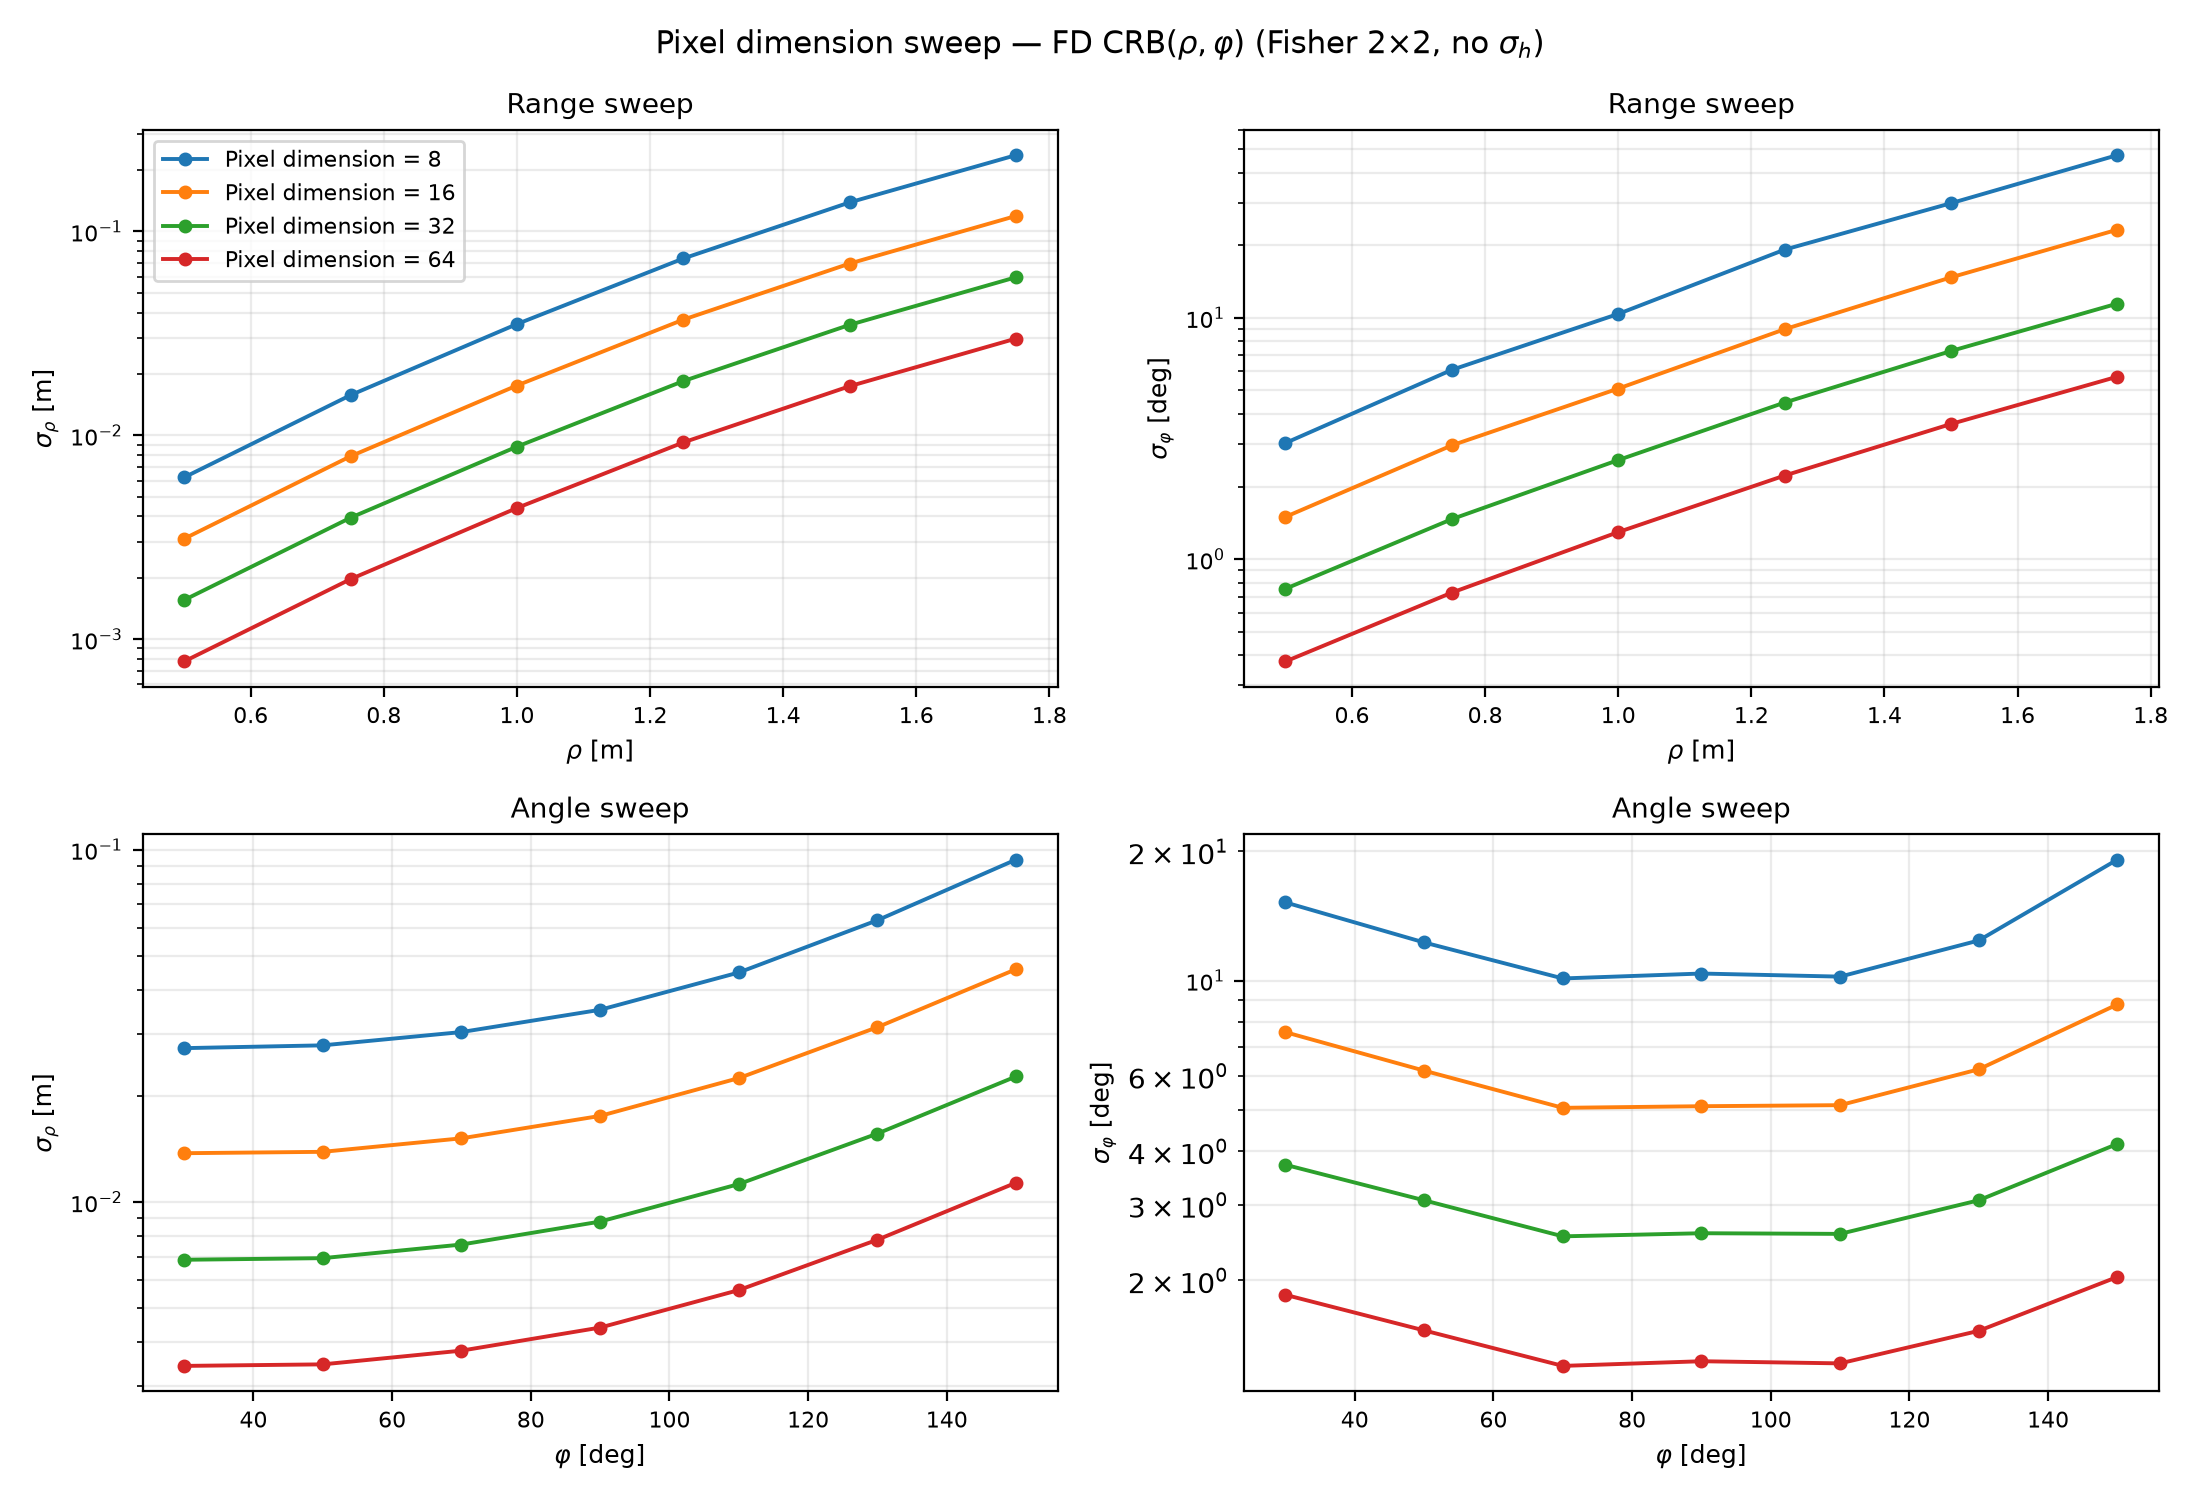
\includegraphics[width=0.98\textwidth]{sr_range_angle_crb.png}}{%
  \fbox{\parbox{0.9\textwidth}{\centering\vspace{2em}(figura
  \code{sr\_range\_angle\_crb.png} no disponible)\vspace{2em}}}}
\caption{Barrido de resolución con \code{sr\_crb.py --pixel-dims 8,16,32,64}.
Arriba: $\sigma_\rho$ y $\sigma_\varphi$ frente a $\rho$ con
$\varphi=90^\circ$ fijo. Abajo: frente a $\varphi$ con $\rho=1\,$m fijo. Las
cuatro curvas de cada panel son paralelas en escala logarítmica y equiespaciadas
por factores de $2$, que es \eqref{eq:escalado}. El crecimiento de
$\sigma_\rho$ con $\rho$ es aproximadamente exponencial en el rango explorado,
consecuencia del $1/(d_1^2d_2^2)$ de \eqref{eq:intensity}.}
\label{fig:sweep}
\end{figure}

\subsection{La rejilla \emph{baseline}}

Con la decisión $N=32$ y el resto de la configuración fijada como la usaba el
repositorio (FOV $0.25\,$m, $\Delta t=3.9\cdot10^{-10}\,$s,
$I_{\text{láser}}=1000$, paredes ocultas, sin ruido, \code{facet.obj} con
$w=0.5\,$m, $b=0.1$, pasos FD $(0.01\,\text{m},0.5^\circ)$), el
\emph{script} \code{compute\_crb\_fd\_baseline.py} evalúa las $15$ poses
$\rho\in\{0.5,1.0,1.5\}\,$m, $\varphi\in\{30,60,90,120,150\}^\circ$.

\begin{table}[htbp]
\centering
\caption{Rejilla \emph{baseline}: CRB$(\rho,\varphi)$ por diferencias finitas
sobre \code{simulator.py} con grilla $32\times32$ y Fisher $2\times2$. No hay
columna $\sigma_h$: no está definida (sección~\ref{sec:limitaciones}).}
\label{tab:baseline}
\begin{tabular}{@{}rr rrrr@{}}
\toprule
$\rho$ [m] & $\varphi$ [$^\circ$] & $\sigma_\rho$ [m]
& $\sigma_\varphi$ [$^\circ$] & $\rho\,\sigma_\varphi$ [m]
& $r_{\rho\varphi}$ \\
\midrule
0.5 & 30 & 0.00136 & 1.0034 & 0.00876 & $-0.731$ \\
0.5 & 60 & 0.00135 & 0.8721 & 0.00761 & $-0.583$ \\
0.5 & 90 & 0.00156 & 0.7535 & 0.00658 & $-0.435$ \\
0.5 & 120 & 0.00222 & 0.8106 & 0.00707 & $-0.402$ \\
0.5 & 150 & 0.00370 & 1.0872 & 0.00949 & $-0.403$ \\
\addlinespace
1.0 & 30 & 0.00685 & 3.7173 & 0.06488 & $-0.564$ \\
1.0 & 60 & 0.00716 & 2.7136 & 0.04736 & $-0.379$ \\
1.0 & 90 & 0.00879 & 2.5741 & 0.04493 & $-0.283$ \\
1.0 & 120 & 0.01318 & 2.6703 & 0.04661 & $-0.250$ \\
1.0 & 150 & 0.02271 & 4.1593 & 0.07259 & $-0.256$ \\
\addlinespace
1.5 & 30 & 0.02566 & 10.7727 & 0.28203 & $-0.452$ \\
1.5 & 60 & 0.02775 & 7.3200 & 0.19164 & $-0.280$ \\
1.5 & 90 & 0.03482 & 7.2896 & 0.19084 & $-0.209$ \\
1.5 & 120 & 0.05176 & 7.3811 & 0.19324 & $-0.191$ \\
1.5 & 150 & 0.09031 & 11.6853 & 0.30592 & $-0.184$ \\
\bottomrule
\end{tabular}
\end{table}

\begin{figure}[htbp]
\centering
\IfFileExists{../plots/crb_fd_baseline_32.png}{%
  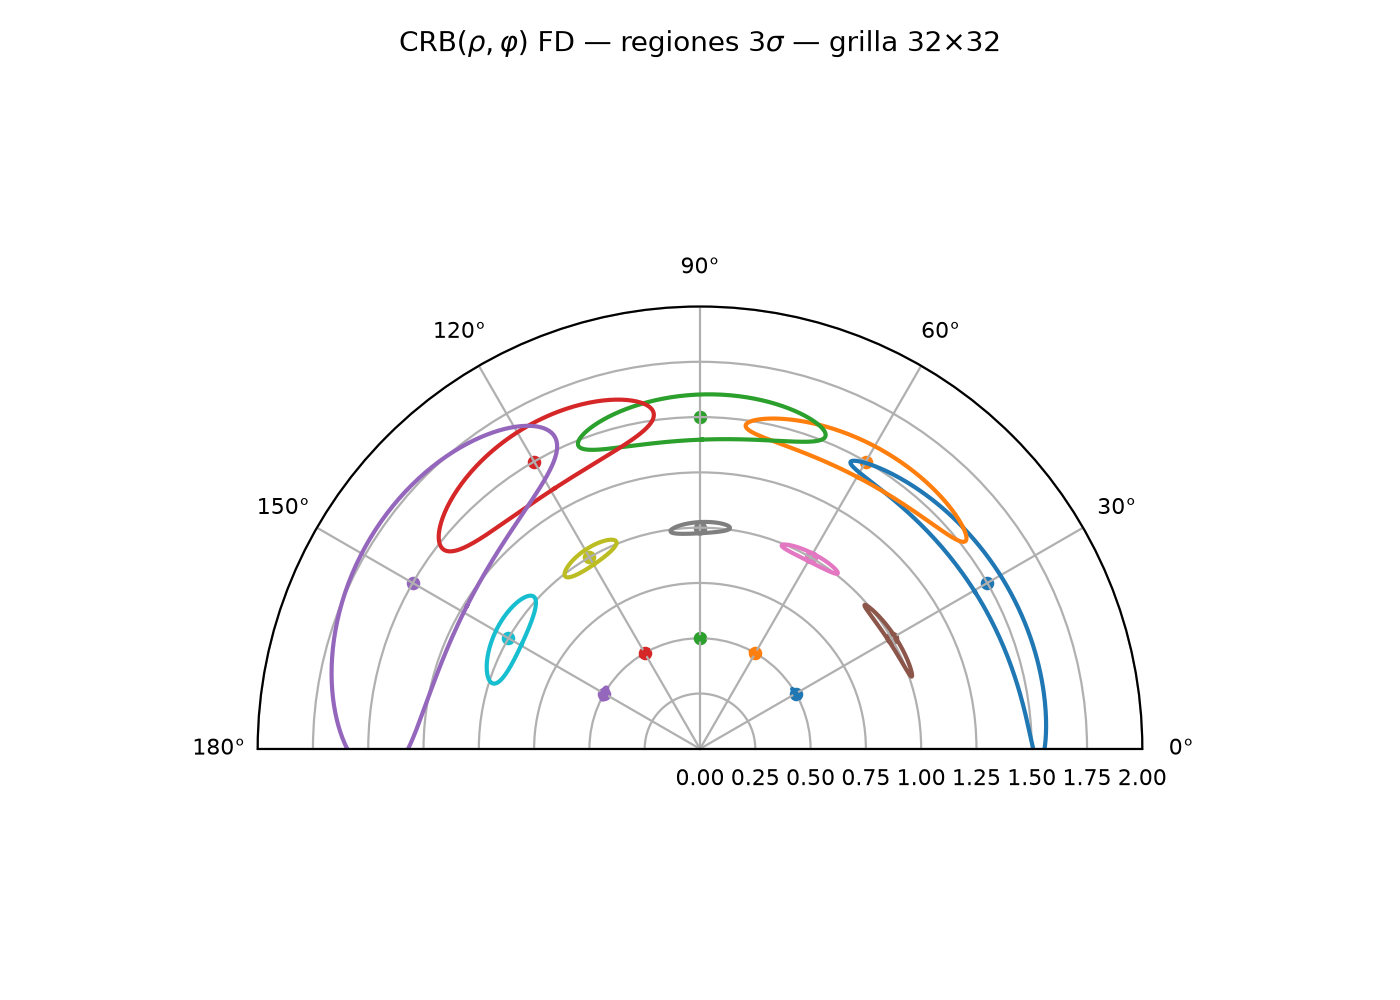
\includegraphics[width=0.74\textwidth]{crb_fd_baseline_32.png}}{%
  \fbox{\parbox{0.9\textwidth}{\centering\vspace{2em}(figura no
  disponible)\vspace{2em}}}}
\caption{Regiones $3\sigma$ del CRB$(\rho,\varphi)$ por diferencias finitas
sobre \code{simulator.py}, grilla $32\times32$. Burbujas en el espacio de
parámetros dibujadas sobre ejes polares, con \code{rlim}$=2.0$. Se regenera con
\code{python3 compute\_crb\_fd\_baseline.py}.}
\label{fig:baseline}
\end{figure}

\subsection{Cómo leer la rejilla}

Cuatro tendencias, todas explicables con lo construido hasta aquí:
%
\begin{itemize}[leftmargin=*]
  \item \textbf{La precisión cae muy rápido con la distancia.} De $\rho=0.5$ a
        $\rho=1.5\,$m, $\sigma_\rho$ crece entre $19$ y $25$ veces según el
        ángulo (de $1.36$ a $25.7\,$mm en $30^\circ$, de $3.70$ a
        $90.3\,$mm en $150^\circ$). El motivo está
        en \eqref{eq:intensity}: la señal decae como $1/(d_1^2d_2^2)$, y con
        varianza igual a la media, menos señal es directamente menos
        información.
  \item \textbf{El ángulo se estima peor en los extremos.} $\sigma_\varphi$ es
        mínima cerca de $\varphi=90^\circ$ y máxima en $30^\circ$ y
        $150^\circ$. En $150^\circ$ la faceta está muy ocluida por la arista
        (en la tabla de la sección~\ref{sec:binning}, solo $105$ de $1024$
        píxeles reciben algo en $(1.5,150^\circ)$), y la información angular la
        aporta precisamente la frontera de la sombra.
  \item \textbf{El error tangencial domina el radial} por un factor entre
        $3.4$ y $6.5$ en todas las poses. La cámara de esquina localiza el rango mucho
        mejor que el azimut: el tiempo de vuelo mide $\rho$ de forma directa,
        mientras que $\varphi$ se infiere indirectamente de la geometría de la
        sombra. Es la anisotropía que produce las elipses muy alargadas.
  \item \textbf{Las correlaciones son todas negativas}
        (sección~\ref{sec:corr}), lo que inclina todas las burbujas en el
        mismo sentido. Su magnitud decrece monótonamente con $\rho$ y, en
        $\varphi$, tiene su mínimo cerca de $120^\circ$ y vuelve a crecer
        ligeramente en $150^\circ$.
\end{itemize}

Comparando con la referencia FD anterior a $64\times64$, la degradación por
bajar a $32\times32$ es un factor $\approx1.9$--$2.4$ en $\sigma_\rho$ y
$\approx1.6$--$1.9$ en $\sigma_\varphi$ sobre la rejilla completa, y
exactamente $2.00$ y $1.99$ en la pose $(1\,\text{m},90^\circ)$ de la
tabla~\ref{tab:sweep}: coherente con \eqref{eq:escalado}, que predice $2$.

%=======================================================================
\section{Mapa del código}
\label{sec:mapa}

{\footnotesize
\newcolumntype{L}[1]{>{\raggedright\arraybackslash}p{#1}}
\begin{longtable}{@{}L{3.5cm}L{5.9cm}L{5.9cm}@{}}
\toprule
Archivo & Función & Etapa de estas notas \\
\midrule
\endfirsthead
\toprule
Archivo & Función & Etapa \\
\midrule
\endhead
\code{simulator.py} & \code{\_transform\_object\_mesh} &
  colocación de la faceta (\S\ref{sec:placement}) \\
& \code{simulate\_transient\_torch} &
  distancias, cosenos, atenuación, oclusión y \emph{binning}
  (\S\ref{sec:distancias}--\S\ref{sec:binning}) \\
& \code{simulation} &
  orquestación, \code{num\_time\_bins}, ruido opcional
  (\S\ref{sec:binning}) \\
& \code{orient\_transient\_} \code{measurement} &
  el \code{roll} de \eqref{eq:roll} (\S\ref{sec:binning} y
  prop.~\ref{prop:roll}) \\
\addlinespace
\code{utils/} \code{densify\_mesh.py} & \code{densify\_mesh\_if\_needed} &
  cuadratura de superficie (\S\ref{sec:placement}) \\
\addlinespace
\code{crb\_fd\_} \code{baseline.py} & \code{simulation\_fn\_for\_crb} &
  adaptador de $2\to3$ valores (\S\ref{sec:adaptador}) \\
& \code{baseline\_simulation\_kwargs}, \code{BASELINE\_*} &
  configuración \emph{baseline} (\S\ref{sec:baseline}) \\
\addlinespace
\code{crb\_polar\_} \code{functions.py} & \code{forward\_g\_polar} &
  $\vect g=\vect y+b$, ec.~\eqref{eq:g} (\S\ref{sec:estadistico}) \\
& \code{finite\_difference\_} \code{jacobian\_polar} &
  jacobiano FD, ec.~\eqref{eq:fd} (\S\ref{sec:fd}) \\
& \code{fisher\_poisson} &
  $\matr I=\matr J^\top\!\operatorname{diag}(1/\vect g)\matr J$,
  ec.~\eqref{eq:fisher-mat} (\S\ref{sec:fisher}) \\
& \code{compute\_crb\_polar} &
  $\matr C=\matr I^{+}$, las $\sigma$ y la correlación (\S\ref{sec:crb}) \\
& \code{crb\_region\_in\_} \code{polar\_parameters} &
  elipse, ec.~\eqref{eq:ellipse} (\S\ref{sec:elipse}) \\
& \code{crb\_region\_physical\_} \code{xy\_to\_polar} &
  empuje a $xy$, ec.~\eqref{eq:pushforward} (\S\ref{sec:elipse}) \\
& \code{plot\_crb\_regions\_polar}, \code{\_style\_polar\_crb\_ax} &
  dibujo de las burbujas (\S\ref{sec:elipse}) \\
\addlinespace
\code{compute\_crb\_} \code{fd\_baseline.py} & \code{main} &
  rejilla de $15$ poses y figura~\ref{fig:baseline} (\S\ref{sec:baseline}) \\
\code{sr\_crb.py}, \code{utils/crb\_utils.py} &
  \code{run\_sweep}, \code{plot\_range\_angle\_sweep} &
  barrido de resolución, tabla~\ref{tab:sweep} (\S\ref{sec:baseline}) \\
\addlinespace
\code{plot\_simulator\_} \code{components.py} & --- &
  figuras \ref{fig:geometria}, \ref{fig:cosenos}, \ref{fig:oclusion},
  \ref{fig:binning} y \ref{fig:transitorio} \\
\code{plot\_binning\_} \code{smoothing.py} & --- &
  figura~\ref{fig:suave} \\
\code{docs/figs\_forward/} \code{make\_aux\_figs.py} & --- &
  figuras \ref{fig:esquema} y \ref{fig:cuantizacion} \\
\bottomrule
\end{longtable}}

%=======================================================================
\section{Limitaciones y salvedades}
\label{sec:limitaciones}

Recogemos aquí, en un solo lugar, todo lo que el \emph{pipeline} no hace, para
que ningún número de estas notas se lea con más autoridad de la que tiene.

\begin{enumerate}[leftmargin=*]
  \item \textbf{No hay altura: el CRB es de dos parámetros y no existe
        $\sigma_h$.} El simulador escala la malla con \eqref{eq:escala} y
        \textbf{nunca lee una clave \code{h}}. La altura de la faceta es un
        resultado de la geometría del \code{.obj} y de $w$, no una entrada
        controlable, así que no existe $\partial\vect g/\partial h$ y la Fisher
        es $2\times2$. El \emph{pipeline} lo impone con
        \code{estimate\_height=False}. Recuperar $\sigma_h$ exigiría
        \emph{añadir} una entrada de altura al simulador, lo que sería un cambio
        de diseño y no una adaptación. Toda la familia de resultados
        \enquote{CRB$(\rho,\varphi,h)$ / Fisher $3\times3$} que aparecía en
        versiones anteriores del estudio ya no es calculable.
  \item \textbf{El jacobiano es una diferencia finita sobre un \emph{forward}
        escalonado} (\S\ref{sec:fd}). Funciona por promediado, no porque el
        modelo sea diferenciable; el resultado tiene una dependencia residual
        del paso y no admite las garantías habituales de convergencia. La
        alternativa con derivadas exactas es la ruta analítica documentada en
        \code{docs/reporte\_consolidado.pdf}, que suaviza $\lceil\cdot\rceil$,
        el indicador y los $\max(0,\cdot)$, deriva en \code{sympy} y reproduce a
        esta ruta dentro de un 10\% en ambos ejes.
  \item \textbf{La oclusión se decide por centroide} y con una pared de medio
        plano infinito (\S\ref{sec:oclusion}, salvedad~\ref{sal:centroide}). No
        hay visibilidad parcial de triángulos ni geometría real del oclusor.
  \item \textbf{No hay supermuestreo dentro del píxel.} La radiancia se evalúa
        en el centro del píxel, sin integrar sobre su huella, con las dos
        consecuencias de la salvedad~\ref{sal:escalado}: los bordes de sombra se
        resuelven al límite de la grilla y el escalado con $N$ es el del modelo,
        no el físico.
  \item \textbf{La suma sobre triángulos es una cuadratura} (\S\ref{sec:placement}).
        Con $32\,768$ triángulos el error es pequeño, pero no nulo, y depende de
        la pose.
  \item \textbf{El modelo de detector es ideal}: Poisson independiente, sin
        tiempo muerto, \emph{pile-up}, diafonía ni \emph{jitter}
        (\S\ref{sec:estadistico}). El CRB resultante es optimista frente a un
        SPAD real.
  \item \textbf{El CRB es una cota local para estimadores insesgados}
        (\S\ref{sec:crb}). No es el error de ningún estimador concreto y no
        captura ambigüedades globales.
  \item \textbf{El plano de la elipse tiene unidades mixtas}
        (salvedad~\ref{sal:unidades}): semiejes e inclinación son convenciones
        consistentes, no invariantes geométricos.
  \item \textbf{Detalles heredados que conviene no idealizar}: el \emph{pitch}
        de $1.57$ en lugar de $\pi/2$ (obs.~\ref{obs:pitch157}), la cota de
        altura inerte (obs.~\ref{obs:altura}) y el \code{roll} de orientación,
        que es una corrección empírica de índice --- inofensiva para el CRB por
        la proposición~\ref{prop:roll}, pero no una operación físicamente
        motivada.
\end{enumerate}

\end{document}
